%Definition des informations du document
\documentclass[a4paper,12pt]{article}
\title{Projet de programmation - QR code dynamique\\Cahier des besoins}
\author{Theo El Houlali, Alexis Henquinet, Thomas Barillot,\\Bourhanoudine Mamodhoussen, Thierno Amadou Diallo, Dimitri Didier
}

%Définition des marges etc..
\setlength{\hoffset}{-18pt}        
\setlength{\oddsidemargin}{9pt} % Marge gauche sur pages impaires
\setlength{\evensidemargin}{9pt} % Marge gauche sur pages paires
\setlength{\marginparwidth}{54pt} % Largeur de note dans la marge
\setlength{\textwidth}{481pt} % Largeur de la zone de texte (17cm)
\setlength{\voffset}{-18pt} % Bon pour DOS
\setlength{\marginparsep}{7pt} % Séparation de la marge
\setlength{\topmargin}{0pt} % Pas de marge en haut
\setlength{\headheight}{0pt} % Haut de page
\setlength{\headsep}{0pt} % Entre le haut de page et le texte
\setlength{\footskip}{27pt} % Bas de page + séparation
\setlength{\textheight}{708pt} % Hauteur de la zone de texte (25cm)

%Import des différents package
\usepackage{graphicx}
\usepackage[T1]{fontenc}
\usepackage[utf8]{inputenc}
\usepackage[francais]{babel}
\usepackage{amsfonts,amsmath,amssymb}
\usepackage{fancyhdr}
\usepackage{stmaryrd}
\usepackage{eqnarray}
\usepackage{tikz}
\usepackage[hidelinks]{hyperref}
\usepackage[many]{tcolorbox}
\usepackage{booktabs}
\usepackage{listings}
\usepackage{titlesec}
\usepackage{mathrsfs}

\usepackage{float}
\usepackage{longtable}

%Réglages de l'en-tête et du pied de page
\renewcommand{\headrulewidth}{0.5pt}
\renewcommand{\footrulewidth}{0.5pt}

%Définition des commandes et des environnements
\newcommand\saut[1]{\vspace{#1\baselineskip}}

\newcommand\Land[0]{\bigwedge}
\newcommand\Lor[0]{\bigvee}
\newcommand\prive[0]{\setminus}

\setcounter{secnumdepth}{4}
\titleformat{\paragraph}
{\normalfont\normalsize\bfseries}{\theparagraph}{1em}{}
\titlespacing*{\paragraph}
{0pt}{3.25ex plus 1ex minus .2ex}{1.5ex plus .2ex}


\newtcolorbox{theoreme_bis}[1]{
    tikznode boxed title,
    enhanced,
    arc=0mm,
    interior style={white},
    attach boxed title to top center= {yshift=-\tcboxedtitleheight/2},
    colbacktitle=white,coltitle=black,
    boxed title style={size=normal,colframe=white,boxrule=0pt},
    title={#1}}
    
\newenvironment{encadre}[1]
{
\begin{theoreme_bis}{#1}
}
{
\end{theoreme_bis}
}

%contenu du document

\begin{document}


\begin{titlepage}
  \begin{sffamily}
  \begin{center}
	
\includegraphics[scale=0.2]{universite.jpg}~\\[1cm]

    \textsc{\Large Projet de programmation - QR code Dynamique }\\[1.5cm]
    Sujet proposé par : Serge Chaumette\\
    Chargé de TD : Boris Mansencal

    % Titre
    \rule{1\linewidth}{2pt}
     \\[1cm]
    { \huge \bfseries Mémoire de Projet de Programmation\\[1cm] }
    \rule{1\linewidth}{2pt}
    \\[3cm]
    
\includegraphics[scale=1]{qr.png}
    \\[1cm]

    % Membres du groupe
   \vfill
      \begin{center}
        Théo El Houlali \hspace*{3.1cm} Thierno Amadou Diallo \hspace*{1.1cm} Thomas Barillot\\
        Bourhanoudine Mamodhoussen \hspace*{1cm} Alexis Henquinet \hspace*{2cm} Dimitri Didier
      \end{center}
 
    % Bas de la page
 
  \end{center}
  \end{sffamily}
\end{titlepage}

\newpage

%\renewcommand{\contentsname}{Sommaire}
\tableofcontents
\newpage

% BOF! Remarque générale : Faut mettre les noms de toutes les fonctions/fichiers en anglais dans le git + dans les diagrammes/textes de ce rapport.

\section{Introduction}


\noindent L'objectif de ce projet est de mettre en œuvre un système de QR codes dynamiques, c'est-à-dire que son contenu évolue au cours du temps. Cela permet par exemple de donner au QR code une durée de vie limitée et/ou de modifier son contenu suivant des paramètres.\\

\noindent Ces paramètres peuvent être l'heure de la journée, un jour de la semaine, mais on peut aussi imaginer des paramètres non-temporels comme la météo ou le nombre de voitures sur un parking (la génération et/ou l'obtention de ces informations ne font pas partie du sujet).\\

\noindent Un exemple d'utilisation pourrait être : un QR code dynamique affiché sur le site web d'une entreprise, qui une fois scanné déclenche un appel téléphonique vers un numéro de garde qui varie selon les plages horaires.\\

\noindent Ce concept de dynamisme devra être paramétrable au moyen de \textbf{plugins} : un court programme fournit par l'exploitant qui définit le contenu du QR code. Nous le verrons plus tard mais idéalement, ce plugin devrait être la seule partie du système que l'exploitant doit écrire.\\

\noindent En quelques mots, nous devons fournir à l'exploitant un moyen \textbf{simple, léger et fiable} de :
\begin{itemize}
\item Paramétrer la génération de ces QR codes dynamiques.
\item Les utiliser sur internet en les intégrant sur une page web.
\item Les utiliser dans un cadre local en les affichant à l'écran d'un ordinateur.\\
\end{itemize}

\subsection{Définitions}
\begin{itemize}

    \item \textbf{QR code} : C'est un type de code barre en deux dimensions constitué de modules noirs disposés dans un carré à fond blanc (un exemple de QR code est présent sur la page de garde). Il peut être scanné dans n'importe quelle direction grâce à ses motifs de détection de position (des "yeux"), situés dans trois des coins. Le QR code est aujourd'hui utilisé pour rediriger vers un site web, un numéro de téléphone, faciliter la connexion vers une borne WiFi, initier un paiement...\footnote{Source : \url{https://www.qrcode.com/en/about/howtouse.html} (consulté le 12/02/2021)}\\

    \item \textbf{Version d'un QR code} : "Version" est un terme qui peut porter à confusion. C'est le terme officiel pour la "taille" d'un QR code\footnote{Source : \url{https://www.qrcode.com/en/about/version.html} (consulté le 12/02/2021)}. Un QR code est composé de modules. On peut imaginer un module comme un pixel dont la valeur binaire est définie par sa couleur (noir ou blanc). Un QR code en version 1 a pour taille 21 x 21 modules (soit 21x21 pixels). La taille maximale est la version 40 avec une taille de 177 x 177 modules. Voir figure \ref{fig:versionQR} ci-dessous pour voir comment le nombre de modules augmente avec la version utilisée.\\
    
    \begin{figure}[H]
        \begin{center}
            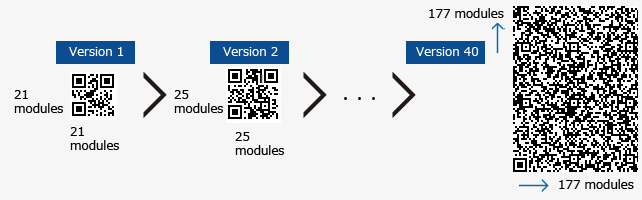
\includegraphics[width=.7\textwidth]{versionVarietyImage.png}
            \caption{On peut voir la taille de différents QR codes en fonction de leur version.\\Source : \url{https://www.qrcode.com/en/about/version.html} (consulté le 12/02/2021)}
            \label{fig:versionQR}
        \end{center}
    \end{figure}
    
    \item \textbf{Niveau de correction d'erreurs d'un QR code} : Les QR codes ont été conçus pour être résistants à la saleté ou l'usure. Cela est possible grâce à l'utilisation du "Code de Reed-Solomon", une méthode également utilisée sur les CD et DVD. Il existe 4 niveaux de correction : L (7\% de correction), M (15\%), Q (25\%) et H (30\%)\footnote{Source : \url{https://www.qrcode.com/en/about/error_correction.html} (consulté le 12/02/2021)}.\\
    
    \item \textbf{Contenu d'un QR code} : Il s'agit tout simplement de l'information obtenue par l'utilisateur scannant le QR code. Nous définissons dans la partie \ref{stadardQR} le type de contenu et en \ref{GenQRCode} la méthode d'encodage de ce contenu.\\
    
    \item \textbf{Dynamisme} : Ici le terme de dynamisme est utilisé pour décrire la logique algorithmique définissant le contenu d'un QR code suivant des paramètres (ex: temporel, valeur retournée par un appel externe, compteur...). Un QR code dynamique est donc un QR code possédant du dynamisme.\\
    
    \item \textbf{Plugin} : Dans le cadre de ce projet, un plugin désigne un programme écrit par l'exploitant lui permettant de définir le dynamisme d'un QR code.\\
    
    \item \textbf{Programme Standalone} : Un programme dédié spécifiquement à l'affichage du QR code. Celui-ci est décrit comme "Standalone" car il est capable de fonctionner par lui même (ne nécessite pas de serveur web, autres infrastructures lourdes...). L'affichage du QR code se limite donc à l'écran de la machine où le programme est exécuté.\\
    
    \item \textbf{Exploitant} : L'exploitant est la personne qui utilisera le système de QR code dynamique pour transmettre des informations aux utilisateurs (ceux qui scanneront les QR codes). Dans notre situation l'exploitant serait vraisemblablement notre client M. Serge Chaumette.\\

\newpage
\subsection{Standard QR code}

\label{stadardQR}

Le QR code doit être bien contrasté, avec un fond clair, posséder une "zone calme" (un contour de la même couleur que le fond tout autour du QR code). La quantité maximale de données stockées est également bornée : environ 3.6 Ko \footnote{La taille maximale est la version 40, 177 * 177 positions, soit 31 329 bits ou environ 3.9 Ko, et le niveau de correction d'erreur minimal est de 7\% donc environ 3.6 Ko. La valeur réelle dépend en réalité de type d'encodage utilisé : 7 089 caractères en encodage numérique, 4 296 en encodage alphanumérique, 2953 caractère en encodage ASCII-étendu et 1817 caractère en encodage Shift JIS.}.\\

Le contenu d'un QR code est toujours une chaîne de caractères (sauf utilisation particulière). Par exemple un texte comme "Hello world" ou une URL comme "https://google.fr" sont encodés de la même manière. C'est le lecteur de QR code qui va interpréter "l'URL" comme telle. 

Pour étendre les fonctionnalités du QR code, un certain nombre de structures de contenu ont été définies au fil des années. On peut voir un liste des structures de contenu (les plus répandues) supportées par les QR codes sur la figure \ref{fig:listStructureContent}.


\begin{figure}[H]
    \begin{center}
        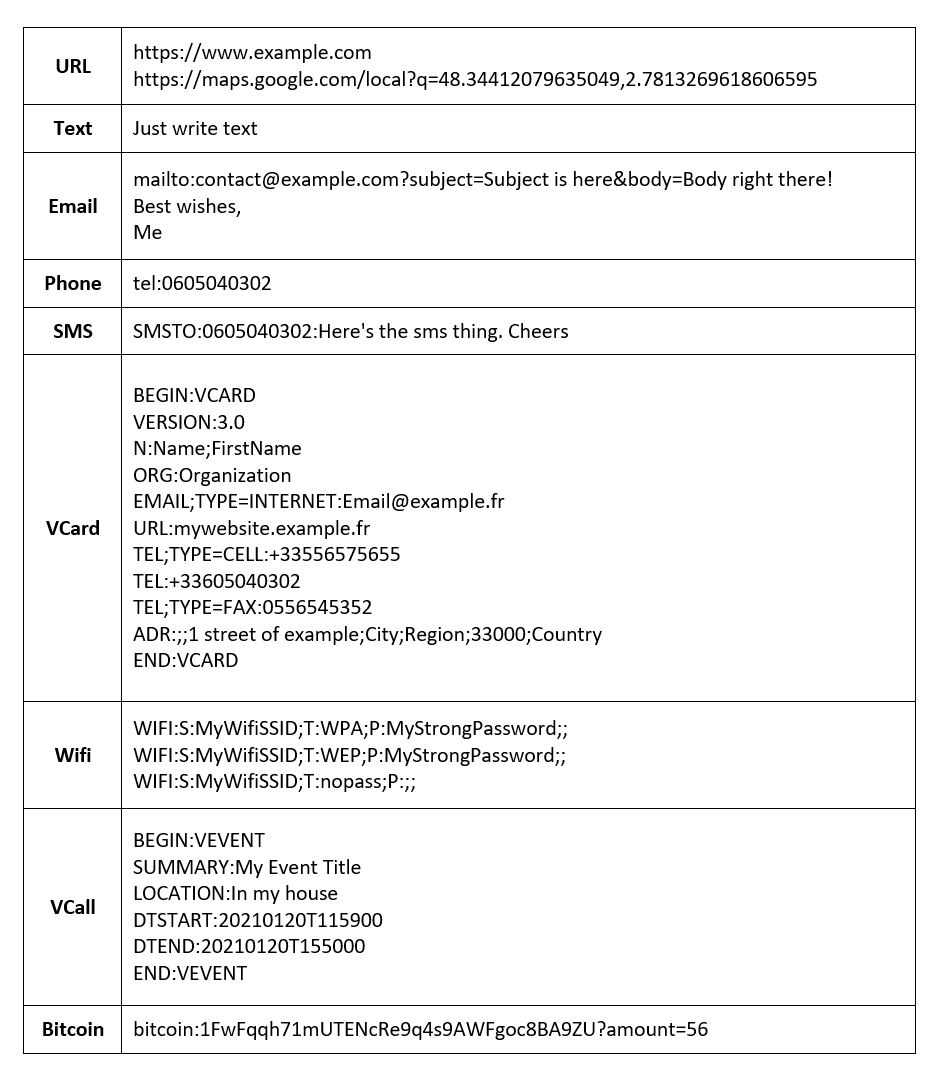
\includegraphics[width=.6\textwidth]{possible to do with QrCode.JPG}
        \caption{Liste des structures de contenu les plus répandues et supportées par les QR codes.\\Source : \url{https://github.com/zxing/zxing/wiki/Barcode-Contents} (consulté le 12/02/2021)}
        \label{fig:listStructureContent}
    \end{center}
\end{figure}

\end{itemize}
\section{Étude de l'existant}

\iffalse % Multi-line comment 
\subsection{Pseudo-code du client}



Nous n'avons pas d'architecture logicielle de base pour ce projet, cependant notre client nous a fourni un pseudo-code d'exemple de plugin non définitif que voici :\\

\begin{lstlisting}
---global time_slot[]=...
global phone_number[]=...

QRcodeContentGenerator(){

time = getTime()
for in in 1, max_time_slots
if (time in time_slot[i])
    return (phone_number[i], CONTENT_TYPE_PHONE_NUMBER)
}
\end{lstlisting}

Ce pseudo-code se rapproche d'un langage Python ou Java. Les deux tableaux en global contiendraient les tranches horaires et les numéros de téléphones associés à générer dans les QR codes dynamiques.\\
Notre client nous as précisé que ce plugin n'est qu'une approche de ce qu'il aimerait obtenir.

\fi % End multi-line comment 

\subsection{Systèmes similaires aboutis}
\noindent L'idée de lier QR code et dynamisme n'est pas quelque chose de nouveau.\\
Une rapide recherche sur internet nous présente de nombreux liens présentant ou vendant ce type de service :\\

\begin{itemize}

    \item \textbf{uQR.me} (\url{https://uqr.me/qr-code-generator} (consulté le 12/02/2021)):\\
    uQR.me est un service payant de création de QR code dynamique par redirection (le QR code est statique et renvoie vers un serveur de redirection web. Le dynamisme a lieu au niveau de cette page de redirection. Voir le tableau dans la partie \ref{compApproches} pour plus de détails). uQR.me semble cibler principalement les entreprises ou organisations qui souhaitent utiliser des QR codes au sein de leur campagne publicitaire. Le service propose la création en quelques clics de QR codes dynamiques pour divers usages. Le prix varie de \$4,95 par mois pour 2 QR codes, à \$49,95 par mois pour 1 000 QR codes. Nous suspectons que ce service ne conviendrait pas à notre client car celui-ci veut pouvoir écrire un script définissant le dynamisme des QR code dynamique (les plugins). L'interface ici se veut très accessible et il n'est pas question d'écrire des lignes de code. Nous pensons donc que uQR.me n'est pas adapté de part sa simplicité qui est ajustée pour un usage grand public. Nous suspectons qu'aucun service en ligne ne permettra l'utilisation de scripts écrits par l'utilisateur à cause des risques d'exécution de code arbitraire\footnote{Code arbitraire est employé pour nommer une action à faire faire à une machine sans que le propriétaire soit d'accord. Plus d'info : \url{https://en.wikipedia.org/wiki/Arbitrary\_code\_execution} (consulté le 12/02/2021)}.\\
    
    \item \textbf{qrd°by} (\url{https://qrd.by/#dynamic-qr-code} (consulté le 12/02/2021)):\\
    qrd°by offre un service payant similaire à uQR.me. Il s'agit là encore de QR codes dynamiques par redirection, ciblant des agences de marketing et entreprises souhaitant lancer une campagne publicitaire. Plusieurs fonctionnalités sont proposées notamment la possibilité de programmer des redirections différentes suivant l'heure de la journée. Le prix de l'abonnement varie entre gratuit (1 QR code et 100 scans par jour), à 35€ par mois (500 QR codes, nombre de scans illimités). Le service souffre malheureusement du même problème soulevé pour le service précédent : le client sera très vite limité par l'interface de création de QR code lorsqu'il souhaitera avoir un usage qui ne rentre pas dans les usages prédéfinis par le site.\\
    
    \item \textbf{DynQR} (\url{https://github.com/bn4t/dynamic-qr} (consulté le 12/02/2021)):\\ 
    DynQR est un service web écrit par Benjamin Nater en Go. Le code source est disponible sur GitHub, sous licence GPL-3.0. DynQR se décrit comme un service web très simple et léger permettant de créer des QR codes par redirection. Il n'y a pas de page de connexion, tout le monde peut créer des QR codes dynamiques. Le système ne propose qu'un type de contenu pour les QR codes : des liens URL. Également, il n'est pas possible de programmer le comportement du QR code dans le temps, la modification du contenu se fait manuellement. Ce programme ne correspond donc pas du tout au besoin de client mais pourrait tout de même être une bonne base si on implémente l'approche de dynamisme par redirection. Le dépôt a été créé en décembre 2019 et a été mis à jour pour la dernière fois en janvier 2021.\\
    
    \item \textbf{PHP Dynamic Qr code}\\(\url{https://github.com/giandonatoinverso/PHP-Dynamic-Qr-code}\\
    (consulté le 12/02/2021)): PHP Dynamic Qr code offre un service web maintenu par Giandonato Inverso et est disponible sur GitHub sous licence MIT. Il offre un service beaucoup plus complet que DynQR, se rapprochant déjà plus des services payants comme uQR.me et qrd°by. Il est possible de créer un grand nombre de QR codes types, personnaliser l'apparence du QR code, son niveau de correction d'erreur, sa taille. Il propose également un tableau de bord permettant de créer, modifier, et voir le nombre de scans pour chaque QR code. L'interface est facile à utiliser et visuellement aboutie. Une démonstration est disponible ici \url{https://www.giandonatoinverso.it/qrcode/} (consulté le 12/02/2021). Tout comme DynQR, il ne semble pas possible de programmer le dynamisme des QR codes, mais juste d'effectuer des modifications manuelles sur le type de redirection. Le dépôt a été créé le 8 septembre 2020 et n'a pas été mis à jour depuis.\\
    
    \item \textbf{A.M.C. System} (\url{https://github.com/hardeepnarang10/attendance-automation} (consulté le 12/02/2021)): A.M.C. System est un système d'apparence complexe, permettant de noter la présence des étudiants aux cours. Le système est développé en Python par Hardeep Narang, disponible sur GitHub sous la licence GPL-3.0. C'est un programme intéressant car notre client avait justement évoqué l'idée d'utiliser les QR codes dynamiques pour cet usage précis. Malheureusement A.M.C. System répond à ce seul besoin et donc son fonctionnement est très différent de ce que l'on souhaite pour notre projet : avec  A.M.C., c'est l'étudiant qui génère un QR code avec une application sur son smartphone et le fait scanner à l'entrée des salles de cours. Le dépôt a été créé et mis à jour pour la dernière fois en octobre 2019.\\
    
\end{itemize}
\noindent
De manière générale, nous voyons que peu de services proposent de "programmer" le dynamisme des QR codes, seulement de le modifier manuellement. C'est un usage qui est suffisant pour la plupart des campagnes marketing (la cible numéro 1 de ces services), mais pas dans notre cas. De plus, tous ces services ne proposent que l'approche par redirection et pas par dynamisme intégré (voir le tableau dans la partie \ref{compApproches} pour plus de détails). Aucun service que nous avons trouvé ne propose l'utilisation de plugins pour définir le dynamisme avec beaucoup plus de contrôle.
\subsection{Bibliothèques}
\noindent Quelle que soit l’approche, il est nécessaire de générer des images de QR codes. Nous avons recherché des bibliothèques permettant de simplifier la génération de QR codes sous Python et sous Java (comme expliqué dans la partie besoins, ce sont les deux langages imposés par le client).\\
Pour Python, un des premiers résultats de notre recherche était PyQRCode 1.2.1 (\url{https://pypi.org/project/PyQRCode} consulté le 12/02/2021). La bibliothèque est maintenue par Michael Nooner, est sous licence BSD et la dernière release en date est de Janvier 2016. Nous avons également envisagé la bibliothèque qrcode 6.1 (\url{https://pypi.org/project/qrcode/} consulté le 12/02/2021) maintenue par Lincoln Loop, également sous licence BSD et dont la dernière release est de Janvier 2019. Cependant nous avons trouvé que cette dernière avait un manque de documentation : il y a quelques exemples, mais il manque un vrai document expliquant toutes les options. PyQRCode propose ce type de documentation ici : \url{https://pythonhosted.org/PyQRCode/} (consulté le 12/02/2021). De plus PyQrCode permet de créer plus facilement les QR Codes (la plupart des QR codes peuvent être générés en une à deux lignes).\\
\noindent
Pour Java, nous avons testé la bibliothèque ZXing 3.4.1 (\url{https://github.com/zxing/zxing} consulté le 12/02/2021) maintenue par Sean Owen, distribuée sous licence Apache-2.0 et dont la dernière release date de Septembre 2020. Le choix de cette bibliothèque vient du fait que ZXing semble être actuellement la bibliothèque principalement utilisée pour les QR code en Java. Après recherche, nous émettons l'hypothèse que cette popularité provient du fait que ZXing est utilisé par Google pour l'analyse des code barres dans les images indexées par son moteur de recherche, mais également en tant que lecteur de code barre par défaut sous Android et dans d'autres produits Google\footnote{Source : \url{https://opensource.google/projects/zxing} (consulté le 12/02/2021)}.\\
\noindent
Nous avons comparé les deux bibliothèques dans la partie \ref{performances}.\\
\section{Besoins}

\noindent Les besoins fonctionnels seront classés par l'ordre de priorité d'implémentation :\\
Niveau 1 : priorité élevée.\\
Niveau 2 : priorité intermédiaire.\\
Niveau 3 : priorité faible.

\subsection{Besoins fonctionnels}


\subsubsection{Génération}

\begin{itemize}
  \item \textbf{Générer des QR} : Niveau 1\\
  \label{GenQRCode}
  Les QR codes permettent l'utilisation de nombreuses structures de données/fonctionnalités, nous souhaitons ici avoir au minimum : le lien URL, le numéro de téléphone et le message textuel. Plusieurs contraintes s'imposent : pour l'encodage du contenu, nous allons nous limiter à ceux nativement compatibles avec le standard QR code, à savoir la norme ASCII étendue et le Shift JIS (caractères japonais). Pour la longueur du contenu, la quantité d'information maximale est de 3,9 Ko (soit 4 296 caractères alphanumérique).\\
  Nous nous sommes également posés la question du format d'image à utiliser pour l'exportation des QR codes. Nous avons donc comparé un QR code version 40 (cas limite) de taille 1000x1000 pixels.\\
  L'image exportée au format PNG pèse 5.54 Ko, là où le même QR code exporté au format JPEG pèse 377 Ko. La différence peut être expliquée en partie par le fait que le PNG supporte le mode bitmap, là ou JPEG doit utiliser le mode RGB. Le mode bitmap utilise 1 bit par pixel là où le mode RGB utilise un octet par canal par pixel (soit 24 bits par pixel). Le JPEG semble supporter 1 octet / pixel (mode nuance de gris) mais les bibliothèques que nous avons utilisé ne permettent pas cette option. Le JPEG2000 est une extension de la norme JPEG. Celui-ci permet l'encodage sur 1 bit par pixel mais est très peu supporté sur internet\footnote{D'après canIuse.com, seulement 19\% des internautes utilisent un navigateur compatible avec le JPEG2000. \url{https://caniuse.com/jpeg2000} (consulté le 22/02/2021)}. De plus, le PNG propose une compression sans perte ce qui est préférable pour faciliter le scan du QR code.\\
  Vis-à-vis du SVG, l'avantage est que la taille du fichier généré ne dépend pas de sa résolution. Le SVG est un format d'image vectorielle, c'est-à-dire que l'on ne stocke pas des pixels mais "une recette" permettant de générer l'image à n'importe quelle résolution. Malheureusement ici, le fichier SVG obtenu pèse 47 Ko soit 8 fois plus lourd que le PNG.\\
  D'autres formats existe notamment le WebP, un format d'image publié par Google (mais open source), disponible depuis 2010. D'après le site canIuse.com\footnote{\url{https://caniuse.com/webp} (consulté le 22/02/2021)}, en 2021 92\% des internautes utilisent un navigateur compatible avec ce format. Aucune bibliothèque ne propose d'exporter les QR codes directement dans ce format, si nous voulons l'utiliser nous devrons nous-même convertir les QR codes obtenus vers le format WebP. La taille du fichier obtenue après convertion (en mode sans pertes) du fichier PNG de 5.54 Ko est un fichier WebP de 4.61 Ko soit environ 17\% plus léger.\\
  Une autre approche serait de générer des images avec une correspondance 1:1 entre la taille du QR code et la résolution de l'image. C'est-à-dire que le QR code version 40 (177*177 modules) sera exporté sous la forme d'une image de taille 177*177 pixels. L'avantage est que l'image obtenue pèse 2.75 Ko, qu'il soit au format WebP ou PNG. L'inconvénient est que l'image doit être agrandie pour être scannée (une image de taille 177*177 pixels serait affichée trop petite à l'écran pour être scannée). Cet agrandissement peut utiliser différentes méthodes d'interpolation : interpolation par plus proche voisin, interpolation bilinéaire, interpolation bicubique... (voir figure ci-dessous où nous présentons deux type d'interpolation). D'après canIuse.com\footnote{\url{https://caniuse.com/css-crisp-edges} (consulté le 22/02/2021)}, 96\% des internautes utilisent un navigateur compatible avec l'interpolation par plus proche voisin.
     \begin{figure}[H]
        \centering
        
\includegraphics[width=.5\textwidth]{pixelated.jpg}
        \caption{Les deux images de QR code sont le même fichier PNG de taille 41*41 pixels, agrandies 7.5 fois sur le navigateur web Firefox. A gauche l'image a été agrandie en utilisant l'interpolation par plus proche voisin, et à droite l'interpolation bilinéaire (interpolation par défaut). L'interpolation bilinéaire n'est pas adaptée à ce type d'image car cette technique tente de créer des transitions entres les couleurs des pixels, elle devient donc floue.}
    \end{figure}
  Conclusion pour le format utilisé : nous pensons que PNG est le format d'image le plus adapté pour ce projet. Le WebP offre des fichiers de tailles plus petites mais nécessite une étape de conversion supplémentaire que nous devrons implémenter. Il y a donc un compromis à faire entre temps de calcul et temps de développement / poids de l'image. De plus, la compatibilité est inférieure pour le WebP, celui-ci étant un format relativement jeune comparé au PNG. Dans notre situation, nous sommes satisfaits avec le poids des images PNG, 5.54 Ko étant un poids très faible pour les images publiées sur internet. Nous n'allons pas aller dans les détails mais le protocole réseau GSM (établi en 1982 et utilisé plus tard pour la 2G) a un débit utile de 3 Ko/s ce qui permettrait de télécharger notre image en 1.8 secondes. Par comparaison, la page d'accueil de Google.fr pèse 1.83 Mo (332 fois plus que notre image PNG).\\
  \item \textbf{Configurer la génération des QR codes par le biais de plugins} : Niveau 1\\
  Les plugins sont des programmes écrits par l'exploitant, lui permettant de définir le dynamisme du QR code. Ces programmes devront suivre une forme particulière que nous développerons dans la partie Architecture.\\
\end{itemize}

\subsubsection{Affichage / intégration}
\begin{itemize}
  
  \item \textbf{Rafraîchir le QR code affiché à l'écran} : Niveau 1
  
  Dans le cas de l'approche par dynamisme intégré, la méthode d'affichage doit permettre de rafraîchir le QR code présenté à période régulière. Ce rafraîchissement doit se faire de manière automatique. Pour une utilisation standalone (en local sur l'ordinateur de l'exploitant), il suffit de réexecuter le plugin, générer l'image de QR code et la recharger dans le programme d'affichage. Pour une utilisation web, ce rafraîchissement nécessite d'avoir un code tournant sur l'ordinateur client. Nous utiliserons un court script écrit en JavaScript pour cela. Dans l'éventualité où l'intervalle de rafraîchissement est très faible (ex: 1s), nous pourrons utiliser des systèmes de caches pour limiter la quantité de téléchargement. (voir chapitre \ref{systemesCaches})\\[0.5cm]
  
 
  \item \textbf{Afficher le QR code dynamique dans un programme standalone} : Niveau 1
  Comme indiqué dans le besoin précédent, le programme standalone est un programme qui tourne en local sur l'ordinateur de l'exploitant. Nous pouvons bien sûr imaginer que le moniteur en question est un téléviseur positionné à l'entrée d'un magasin ou d'un bureau (voir les exemples d'utilisations présentés dans l'introduction).\\
  \item \textbf{Intégrer le QR code dynamique sur le site web de l'exploitant} : Niveau 2
  Le site web de l'exploitant tourne sous PHP (ou du moins accepte l'utilisation de code PHP). Dans le cas de l'approche par dynamisme intégré, cela pose une contrainte sur le langage à utiliser pour le dialogue entre la page web et le back-end. Il sera nécessaire de vérifier la compatibilité avec les différents navigateurs web.\\
  \item \textbf{Imprimer les QR codes} : Niveau 3\\
  Ce n'est pas un besoin indiqué par le client. Cependant nous avons jugé utile d'en parler pour mieux définir les avantages et les inconvénients de chaque approche. De part la nature des QR code à dynamisme intégré, il n'est pas possible de les imprimer : il faut un code machine pour modifier le QR code affiché. Ce n'est pas un problème avec le QR code à dynamisme par redirection qui n'est qu'une simple image statique pointant vers une URL. Il existe seulement une contrainte majeure : \textbf{le smartphone de l'utilisateur scannant le QR code doit avoir accès à internet.}\\
  
  \item \textbf{Intégrer un QR code sur n'importe quel site web} : Niveau 3\\
  De même que le besoin précédent, ce n'est pas un besoin indiqué par le client. Pour une utilisation sur le web, l'approche par dynamisme intégré nécessite de déposer du code PHP et JS pour gérer le rafraîchissement des QR codes.\\ Cela restreint leurs utilisations aux sites web dont on est administrateur : il n’est pas possible de les publier sur les réseaux sociaux et autres. Également, bien que PHP soit massivement utilisé sur les serveurs d’hébergement web, il existe d’autres frameworks tel que Asp .Net, Enyo, Ruby on Rails, NodeJs... Pour intégrer les QR codes sur un site utilisant une autre technologie que PHP, il serait nécessaire de réécrire une nouvelle version de l’intermédiaire web.
  Encore une fois, ce n'est pas un problème avec le QR code à dynamisme par redirection.\\
  
\end{itemize}
\subsubsection{Autres fonctionnalités}

\begin{itemize}
  
  \item \textbf{Donner une limite temporelle au QR code} : Niveau 2\\
  Il doit être possible d'indiquer un horodatage auquel le QR code n'est plus visible, ou renvoie un message tel que "Le contenu n'est plus disponible". C'est ici que l'approche par dynamisme intégré a ces limites : dans l’éventualité où un utilisateur télécharge l’image, la prend en photo ou potentiellement la publie, il n’est pas possible d’empêcher quiconque de scanner et de visionner le contenu du QR code. L'approche par redirection permet un réel contrôle d'accès au contenu. Cette différence s'explique par le fait que dans la première approche, le contenu dont on souhaite limiter l'accès se trouve dans le QR code, là où le système par redirection ne fournis que l'URL pour y accéder.\\
  
\end{itemize}

\subsection{Besoins utilisateurs non fonctionnels}

\noindent Avant de commencer cette partie, nous souhaitons indiquer que l'exploitant a émis comme condition que le langage utilisé pour la création des plugins devrait être Python ou Java. C'est pour cela que vous constaterez une dualité entre les deux (et ces deux là seulement) dans les besoins suivants. Nous terminerons par le besoin \textbf{"langages utilisé pour l'écriture des plugins"} qui servira de conclusion aux observations faites dans les autres besoins.\\

\begin{itemize}
  
  \item \textbf{Performances} :\\
  \label{performances}
  Trois aspects peuvent impacter les performances de notre système : le temps de réponse, la vitesse d'exécution et la mémoire utilisée. Nous n'avons défini aucune contrainte avec le client. Nous allons donc nous-même nous fixer des contraintes réalistes en supposant que le système tourne sur du matériel informatique standard\footnote{En opposition avec un serveur de calcul dédié. Les tests ayant été effectué sur un de nos ordinateurs personnels, c'est ce que l'on considèrera comme "du matériel informatique standard". La configuration du PC était un Ryzen 5 2600 (6 coeurs, 12 threads) avec 8 Go de mémoire vive DDR4.}, et que d'autres programmes peuvent également être en fonctionnement sur la machine (on pense notamment à un serveur web).\\
  
  Pour notre premier test, nous avons généré des QR codes de taille 500x500 pixels avec un niveau de correction L et de version "auto" (cela signifie que la bibliothèque sélectionne la version de QR code de taille minimale où la quantité de données fournie peut être stockée). Le contenu était "Ceci est un test de QRCode numéro i" où i varie avec l'indice du QR code en cours de génération. Nous avons généré des lots de quantités différentes (1, 5, 10 , ...). Nous avons choisi ces propriétés car cela correspond à des cas d'utilisation habituelle. Vous pouvez retrouver les algorithmes utilisés dans l'annexe à la fin du document. Voici les résultats ci-dessous :

    \begin{figure}[H]
        \centering
        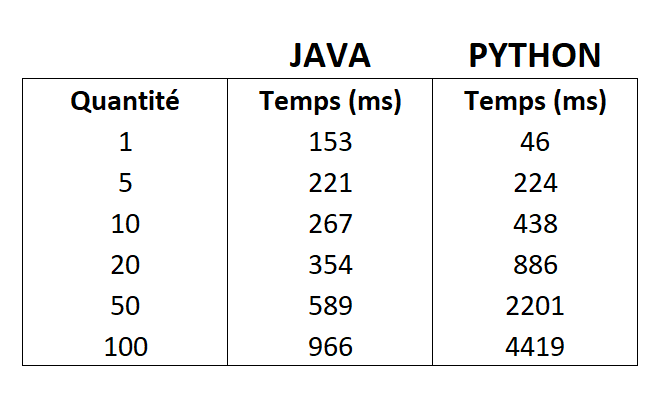
\includegraphics[width=.5\textwidth]{vitesse small.png}
        \caption{On peut voir que Python est presque 3 fois plus rapide pour produire 1 QR code. Cependant, le temps de calcul croit linéairement avec le nombre de QR code pour Python (environ 44 ms/QR code quelle que soit la quantité), là où le Java croit plus lentement (153 ms pour 1 code mais 9.6 ms/QR code pour 100 QR code).}
    \end{figure}
 
  Nous avons fait un second test avec des QR codes "extrêmes" : niveau de correction H (la plus élevée), version 40 (la plus grande), et une résolution de 1000x1000 pixels. Le contenu reste inchangé ainsi que les algorithmes utilisés. Voici les résultats : 
  
  
      \begin{figure}[H]
        \centering
        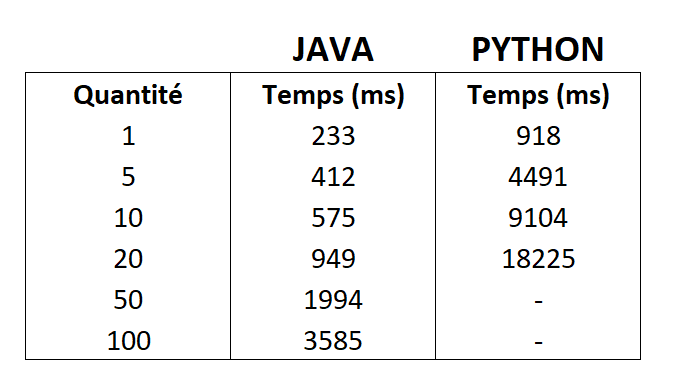
\includegraphics[width=.5\textwidth]{vitesse big.png}
        \caption{On peut voir que Python est presque 4 fois plus lent que Java. Et cet écart ne fait que croître avec la quantité. Nous avons d'ailleurs interrompu le test pour Python pour les quantités 50 et 100 car les temps de calculs étaient trop longs. Java est ici le gagnant incontesté.}
    \end{figure}

    
  Il faut cependant prendre en compte deux paramètres pour correctement interpréter ces résultats vis-à-vis de ce projet : même en générant des QR codes extrêmes (le pire scénario possible), il est possible de générer 1 QR code à la seconde. Au vu de l'utilisation demandée pour ce projet, ces résultats nous paraissent satisfaisants quel que soit le langage choisi.\\
  
  Vis-à-vis de la mémoire vive, la machine virtuelle Java (JRE) consomme 20 Mo à vide (une boucle while sans opération). Lors de la génération de 500 QR codes sur 16 secondes, la consommation est restée parfaitement constante à environ 300 Mo de mémoire vive utilisée. Python lui a une consommation à vide de 10 Mo, et de 15 Mo lors de la génération des QR codes (suivant le même protocole). Python est donc meilleur pour une consommation mémoire faible.\\
    \newpage
  Vis-à-vis de la taille des fichiers produits, la différence est faible : Java produit des fichiers de 6.5 Ko et Python 5.5 Ko pour des images PNG de QR code version 40 et de taille 1000x1000 pixels. Dans tous les cas, ce sont des poids très faibles, similaires à ceux d'une favicon (le logo d'une page web, souvent affiché dans l'onglet à côté du titre de la page).\\
  
  Vis-à-vis du temps de réponse, nous avons essayé de mesurer le temps qu'il faut pour afficher un "Hello world" dans les deux langages. Nous avons mesuré 0.55s pour Java et 0.59 pour Python (moyenne basé sur 10 mesures pour chaque langage). Nous n'avons pas de garantie mais nous pensons que ces temps prennent en compte l'inclusion des bibliothèques. Dans tous les cas ces résultats ne permettent pas de désigner un langage plus performant.\\
  
  Au delà du langage de programmation/bibliothèque utilisé, d'autres questions de performances se posent, notamment si ce système est utilisé au sein d'un site web ayant de nombreux visiteurs en parallèle. Nous avons détaillé ce point dans la \textbf{Partie 5} en expliquant pourquoi des systèmes de caches peuvent réduire considérablement la charge du système.\\

  \item \textbf{Facilité d'utilisation} :\\
  La facilité d'utilisation est un point important pour l'exploitant : il souhaite avoir le moins de code à écrire, c'est-à-dire se limiter à l'écriture des plugins, et possiblement lors de l'installation/configuration initial du système. L'écriture des plugins doit elle aussi être facilitée : nous avons pensé qu'il serait intéressant d'inclure un certain nombre de modèles types. Par exemple, une classe qui permettrait de créer un QR code pour l'envoi de mails (avec des attributs pour la boite de destination, un sujet par défaut, un corps par défaut).\\
  
  Il s'agit de fournir à l'exploitant un "formulaire de création" sous la forme d'attributs de classe. Dans un premier temps nous pourrions créer des classes "formulaire" pour les types \textbf{Text}, \textbf{URL} et \textbf{Phone}, puis d'étendre l'idée aux autres types.\\
  
  Il existe tout de même un risque : en voulant trop simplifier l'écriture des plugins, on risque de limiter les possibilités.\\

  \item \textbf{Fiabilité, sécurité} :\\
  Il est également important de limiter le risque d'erreur : un plugin (code du l'exploitant) ne doit pas pouvoir faire planter le système. Il faudra être capable de mettre en place des sections de code non-modifiables par les plugins, par exemple au moyen d'interfaces, et/ou de classes et objets privés. C'est-à-dire, limiter la capacité des plugins à leur stricte minimum : des fonctions qui génèrent des chaînes de caractère.\\
  
  Vis-à-vis de la fiabilité du système, nous allons bien sûr mettre en place les tests unitaires nécessaires. Le point que nous considérons comme le plus important est de garantir la conformité du contenu du QR code selon ce que le plugin a fourni. Avec les quatre modes d'encodage du QR code, qui possèdent tous des limitations sur les plages ASCII/Unicode compatibles, un problème d'encodage est vite arrivé. Afin de garantir cette conformité, nous proposons de systématiquement vérifier à l'aide d'un décodeur les QR codes générés en comparant le contenu donné en entrée et obtenu en sortie.\\
  
  Ici, le choix du langage a également son importance. Java possède des mots-clés puissant comme final ou private, ainsi qu'un typage fort. Python lui propose plutôt des manières pour indiquer que des attributs sont privés, sans réelles protections. Au moyen de techniques comme la "décoration de nom" ou Name mangling\footnote{Source : \url{https://en.wikipedia.org/wiki/Name_mangling} (consulté le 12/02/2021)} en anglais, il est possible d'accéder et même de modifier des attributs "privés".
  Le langage Java paraît donc le plus approprié pour limiter les capacités d'un plugin à "casser" le système.\\
  
  \item \textbf{Portabilité} : L'installation ou la réinstallation du système doit être rigoureusement documentée. Si possible il doit pouvoir être installé sur Windows ou Linux. Nous ne pourrons pas tester toutes les versions de Windows, et encore moins toutes les branches de Linux. Nous allons donc nous focaliser dans un premier temps sur un système tournant sur Debian 10. Nous verrons plus tard s'il est facile de porter notre système sur une machine tournant sous Windows 10. Nous avons tout de même de bon espoir en terme de portabilité de part l'utilisation de Python qui est un langage interprété, ou bien de Java. Le client est également intéressé pour installer le système d'affichage standalone sur un Raspberry Pi. L'intérêt serait de pouvoir brancher l'appareil à l'arrière d'un écran ou une télévision : moins de fils, faible consommation électrique, pas de bruit.\\
  
  \item \textbf{Le langages utilisé pour l'écriture des plugins} :\\
  Le client souhaite que les plugins soient écrits dans un langage de programmation avec lequel il est familier : Python ou Java.
  Il nous a donc fallu dégager les avantages/inconvénients des deux langages pour déterminer le plus adapté. Nous avons en premier pensé au temps de génération des QR code cependant nos faibles exigences en terme de performance ne permettent pas de déterminer un langage vainqueur (voir le besoin \textbf{Performances} ci-dessus).\\
  
  Nous nous sommes donc penchés sur le sujet de la facilité d'utilisation, que ce soit pour l'exploitant et nous mêmes. Ici Python se démarque par sa simplicité de code (voir la différence de la taille des programmes de tests en annexe), et le fait qu'il s'agisse d'un langage interprété (l'exploitant n'a pas à compiler ses plugins avant utilisation). Encore une fois vous trouverez plus de détails ci-dessus, dans la partie \textbf{Facilité d'utilisation}.\\
  
  Nous avons également étudié la question de la sécurité : quel langage permet de limiter les conséquences d'un plugin présentant des bugs ? Notre analyse montre que Java permet de mieux protéger son code à l'aide de mots clés puissants, de son typage fort et de l'utilisation d'un compilateur qui vérifie des erreurs typiques comme une faute de frappe dans le nom d'une variable. Python ne permet que de fournir des indications sur l'utilisation des attributs d'une classe. Malgré tout, nous pensons que l'utilisation de Python ne poserait pas de réel danger dans la mesure où les plugins ont uniquement accès au pointeur de l'objet de retour de sa fonction getContent(). Cela signifie que l'exploitant ne pourra pas modifier de fonctions/objets utilisés dans le code des autres parties du systèmes. Voir le besoin \textbf{Fiabilité, sécurité} ci-dessus pour plus de détails.\\
  \newpage
  Pour finir, nous nous sommes intéressés aux évolutions futures. Cette fois Python (ou plutôt sa bibliothèque PyQRcode) se démarque grâce aux nombreuses options de personnalisation du QR code proposé, comme par exemple la couleur du fond, la couleur des modules, ou encore la possibilité d'exporter l'image en mode vectoriel.\\
  
  Nous avons donc décidé de choisir Python comme langage pour l'écriture des plugins, et par extension la majorité du système (l'unicité du langage permet de simplifier le dialogue entre les différentes parties du programme).\\
  
\end{itemize}

\section{Scénarios fonctionnels}
\label{architecture}
\subsection{Scénarios}
\label{scenario}
\noindent On retrouve ici les scénarios principaux de notre projet, à savoir la version standalone, la version web et la version redirection web, présentées de manière "vulgarisée" (on rentre pas dans les détails du code pour l'instant).\\

\begin{itemize}
  \item \textbf{QR codes à dynamisme intégré} - Le dynamisme a lieu au niveau de l’affichage du QR code. Le QR code affiché change périodiquement.\\
  \item \textbf{QR codes à dynamisme par redirection} - Le QR code est statique et renvoie vers un serveur de redirection web. Le dynamisme a lieu au niveau de cette page de redirection.\\
\end{itemize}
\noindent
Nous verrons par la suite que les deux approches sont loin d'être incompatibles : il est facile de rajouter la fonctionnalité de dynamisme par redirection à partir d'un système initialement prévu pour le dynamisme intégré.

\subsubsection{Approche utilisant des QR codes à dynamisme intégré}

\paragraph{Liste des parties qui composent ce système}
    \begin{itemize}
  \item \textbf{Plugins} - Un programme écrit par l'exploitant lui permettant de définir le dynamisme d'un QR code.\\
  
  \item \textbf{Fonction orchestratrice} - Prend en paramètres un plugin et un chemin. Le plugin lui fournit le contenu qu'elle transmet à la \textbf{génération de QR code}.\\
  
  \item \textbf{Génération de QR code} - Permet de créer une image PNG ou SVG du QR code à partir d'une chaîne de caractères.\\
  
  \item \textbf{Intermédiaire web} - Gère l'appel au logiciel back-end, fournit le QR code produit à la partie web.\\
  
  \item \textbf{Affichage client web} - Va demander la dernière version du QR code à fréquence régulière à l'\textbf{intermédiaire web}. C'est cette partie qui va permettre au navigateur de toujours présenter à l'utilisateur la dernière version du QR code.\\
  
  \item \textbf{Affichage standalone} - À partir d'un fichier de plugin, affiche le QR code correspondant à l'écran de l'ordinateur.\\

\end{itemize}
\noindent
Voici ci-dessous un schéma permettant de montrer les interactions entre chacune des parties du systèmes et les acteurs. La chronologie des interactions est définie dans les scénarios (\ref{scen:1A} et \ref{scen:1B}).

\begin{figure}[H]
\begin{center}
  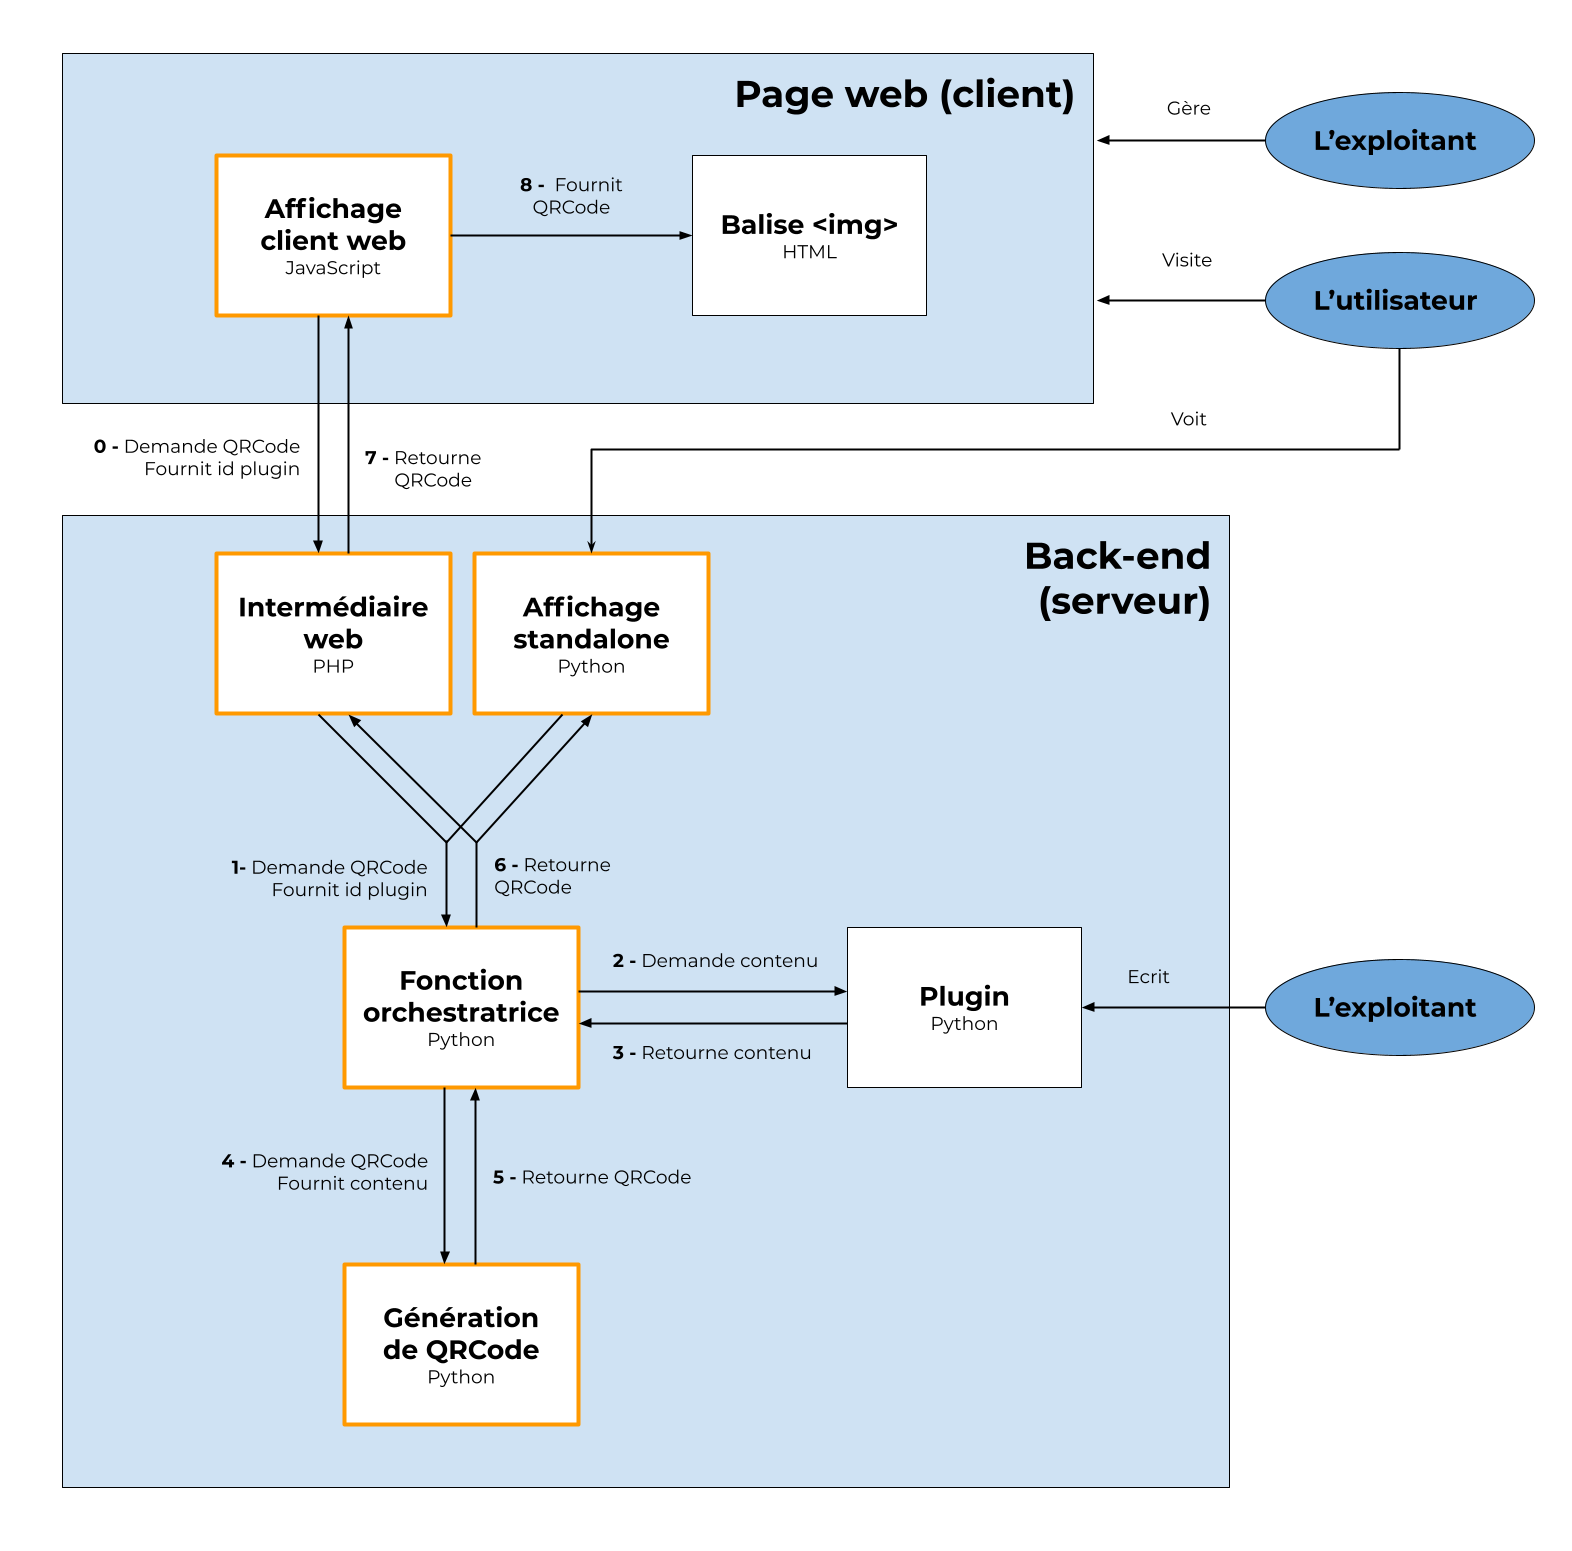
\includegraphics[width=.8\textwidth]{Organigramme QRCode.png}
  \caption{Les ellipses bleu foncées sont les acteurs : l'exploitant et l'utilisateur (qui visite la page web ou se présente devant l'écran de l'affichage standalone). Les rectangles sont les parties du système et ceux entourés en orange sont celles que nous avons codées. C'est-à-dire toutes sauf les balises <img> (qui sont à la charge de l'exploitant d'ajouter sur son site web) et les plugins (qui encore une fois sont écrits par l'exploitant).}
\end{center}
\end{figure}

\paragraph{Scénario A : une requête web}
    \label{scen:1A}
\noindent Afin de présenter comment ces différents systèmes fonctionnent ensemble, regardons l'enchaînement des évènements lorsqu'un client visite une page web contenant un QR code dynamique. Les numéros entre parenthèses correspondent aux numéros d'étapes sur le schéma ci-dessus.\\
  \newpage
\begin{itemize}
  \item Un utilisateur visite la page web.
  \item Le serveur lui fournit le code HTML, CSS, JS.
  \item Une fois la page chargée, (0) l'\textbf{Affichage client web} (fonction JS) fait une requête pour récupérer la dernière version de QR code dynamique au serveur.
  \item (1) L'\textbf{intermédiaire web} (code PHP) reçoit la demande et fait une requête à la \textbf{fonction orchestratrice} (back-end Python) pour obtenir l'image.
  \item (2) La \textbf{fonction orchestratrice} exécute le plugin passé en paramètre et (3) génère donc le contenu pour le QR code. (4) La fonction transmet ensuite le contenu à la fonction de \textbf{génération de QR code} qui produit l'image à l'emplacement souhaité.
  \item (5 et 6) De retour à l'\textbf{intermédiaire web}, (7) celui-ci retourne à l'\textbf{affichage client web} le chemin pour accéder à l'image.
  \item (8) Pour finir l'\textbf{affichage client web} modifie la balise <img> vide pour lui faire afficher l'image. Après une période de temps (qui sera définie par le plugin et transmise par l'\textbf{intermédiaire web}), l'\textbf{affichage client web} réitère l'opération et fait à nouveau une requête (retour à l'étape 1).\\
\end{itemize}

\paragraph{Scénario B : Affichage standalone}
    \label{scen:1B}
\noindent Nous pouvons constater que les parties \textbf{Plugins}, \textbf{Interface}, et \textbf{Génération de QR code} sont communes aux utilisations sur le web et en standalone. Détaillons tout de même le processus en utilisant le même schéma :\\
\begin{itemize}
  \item L'exploitant ouvre l'\textbf{afficheur standalone}.
  \item (1) \textbf{L'affichage standalone} fait une requête pour récupérer la dernière version de QR code dynamique au serveur.
  \item (2) La \textbf{fonction orchestratrice} exécute le plugin passé en paramètre et (3) génère donc le contenu pour le QR code. (4) La fonction transmet ensuite le contenu à la fonction de \textbf{génération de QR code} qui produit l'image à l'emplacement souhaité.
  \item (5 et 6) De retour à l'\textbf{affichage standalone}, celui-ci l'affiche à l'écran.
  \item L'utilisateur se présente devant l'écran de \textbf{l'affichage standalone} et peut le scanner.\\
\end{itemize}


\subsubsection{Approche des QR codes à dynamisme par redirection}


\paragraph{Différence avec l'approche par dynamisme intégré}

\noindent Un système de QR code fonctionnant par redirection dynamique n'est pas très différent d'un système par dynamisme intégré. Les différences principales sont :

\begin{itemize}
  \item Il faut pouvoir générer des QR codes statiques amenant à une page web (il faut donc nécessairement un serveur web).
  \item Dans l'approche par dynamisme intégré, l'afficheur web affiche un QR code dont le contenu est mis-à-jour par un plugin. En dynamisme par redirection, il faut simplement afficher le contenu.
\end{itemize}

\noindent On voit donc qu'au niveau de l'architecture, les deux approches sont très similaires si ce n'est la partie présentation (Afficheur web).

\begin{figure}[H]
\begin{center}
  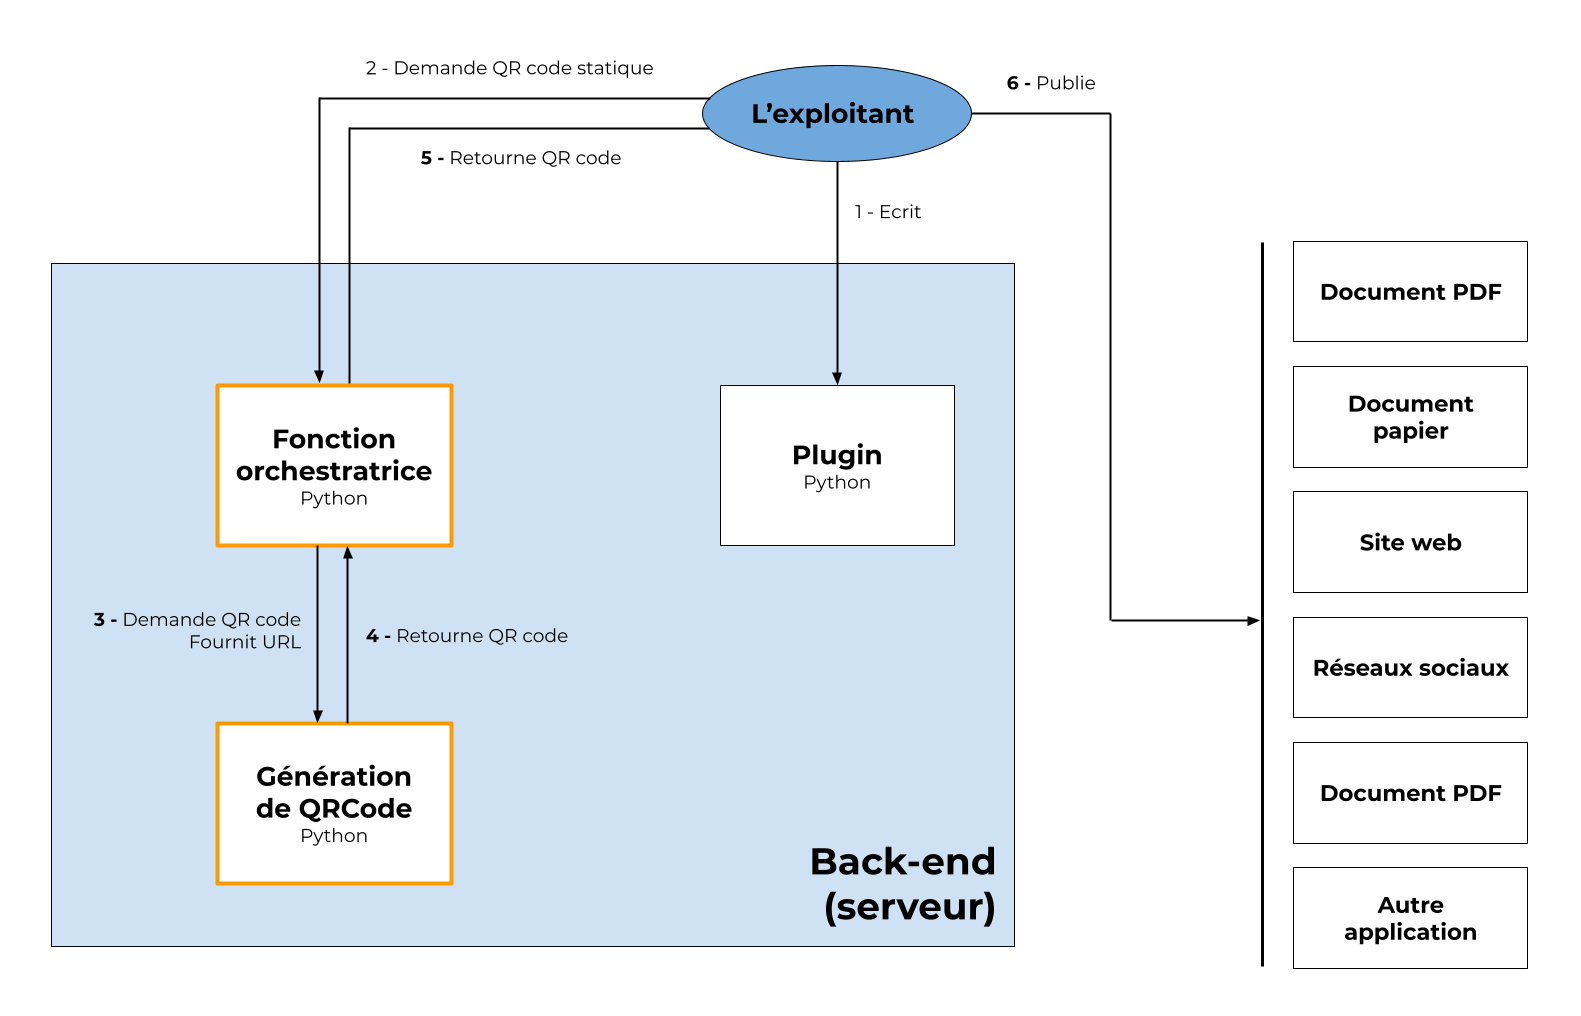
\includegraphics[width=1\textwidth]{Par redirection v2.png}
  \caption{L'ellipse bleu foncée est un acteur. Les rectangles sont les parties du système et ceux entourés en orange sont celles que nous devons coder.}
\end{center}
\end{figure}

\paragraph{Scénario A : création d'un plugin et publication du QR code statique associé}
\begin{itemize}
 \item (1) L'exploitant commence par écrire son \textbf{plugin}.
 \item (2) Il demande ensuite la génération du QR code statique à la \textbf{fonction orchestratrice}
 \item La \textbf{fonction orchestratrice} génère une URL pour chaque plugin, et (3) transmet ces URLs à la fonction de \textbf{génération de QR code} qui (4) produit les QR code statique dans un dossier spécifique.
 \item (5 et 6) L'exploitant peut maintenant partager/publier le QR code.
\end{itemize}

\begin{figure}[H]
\begin{center}
  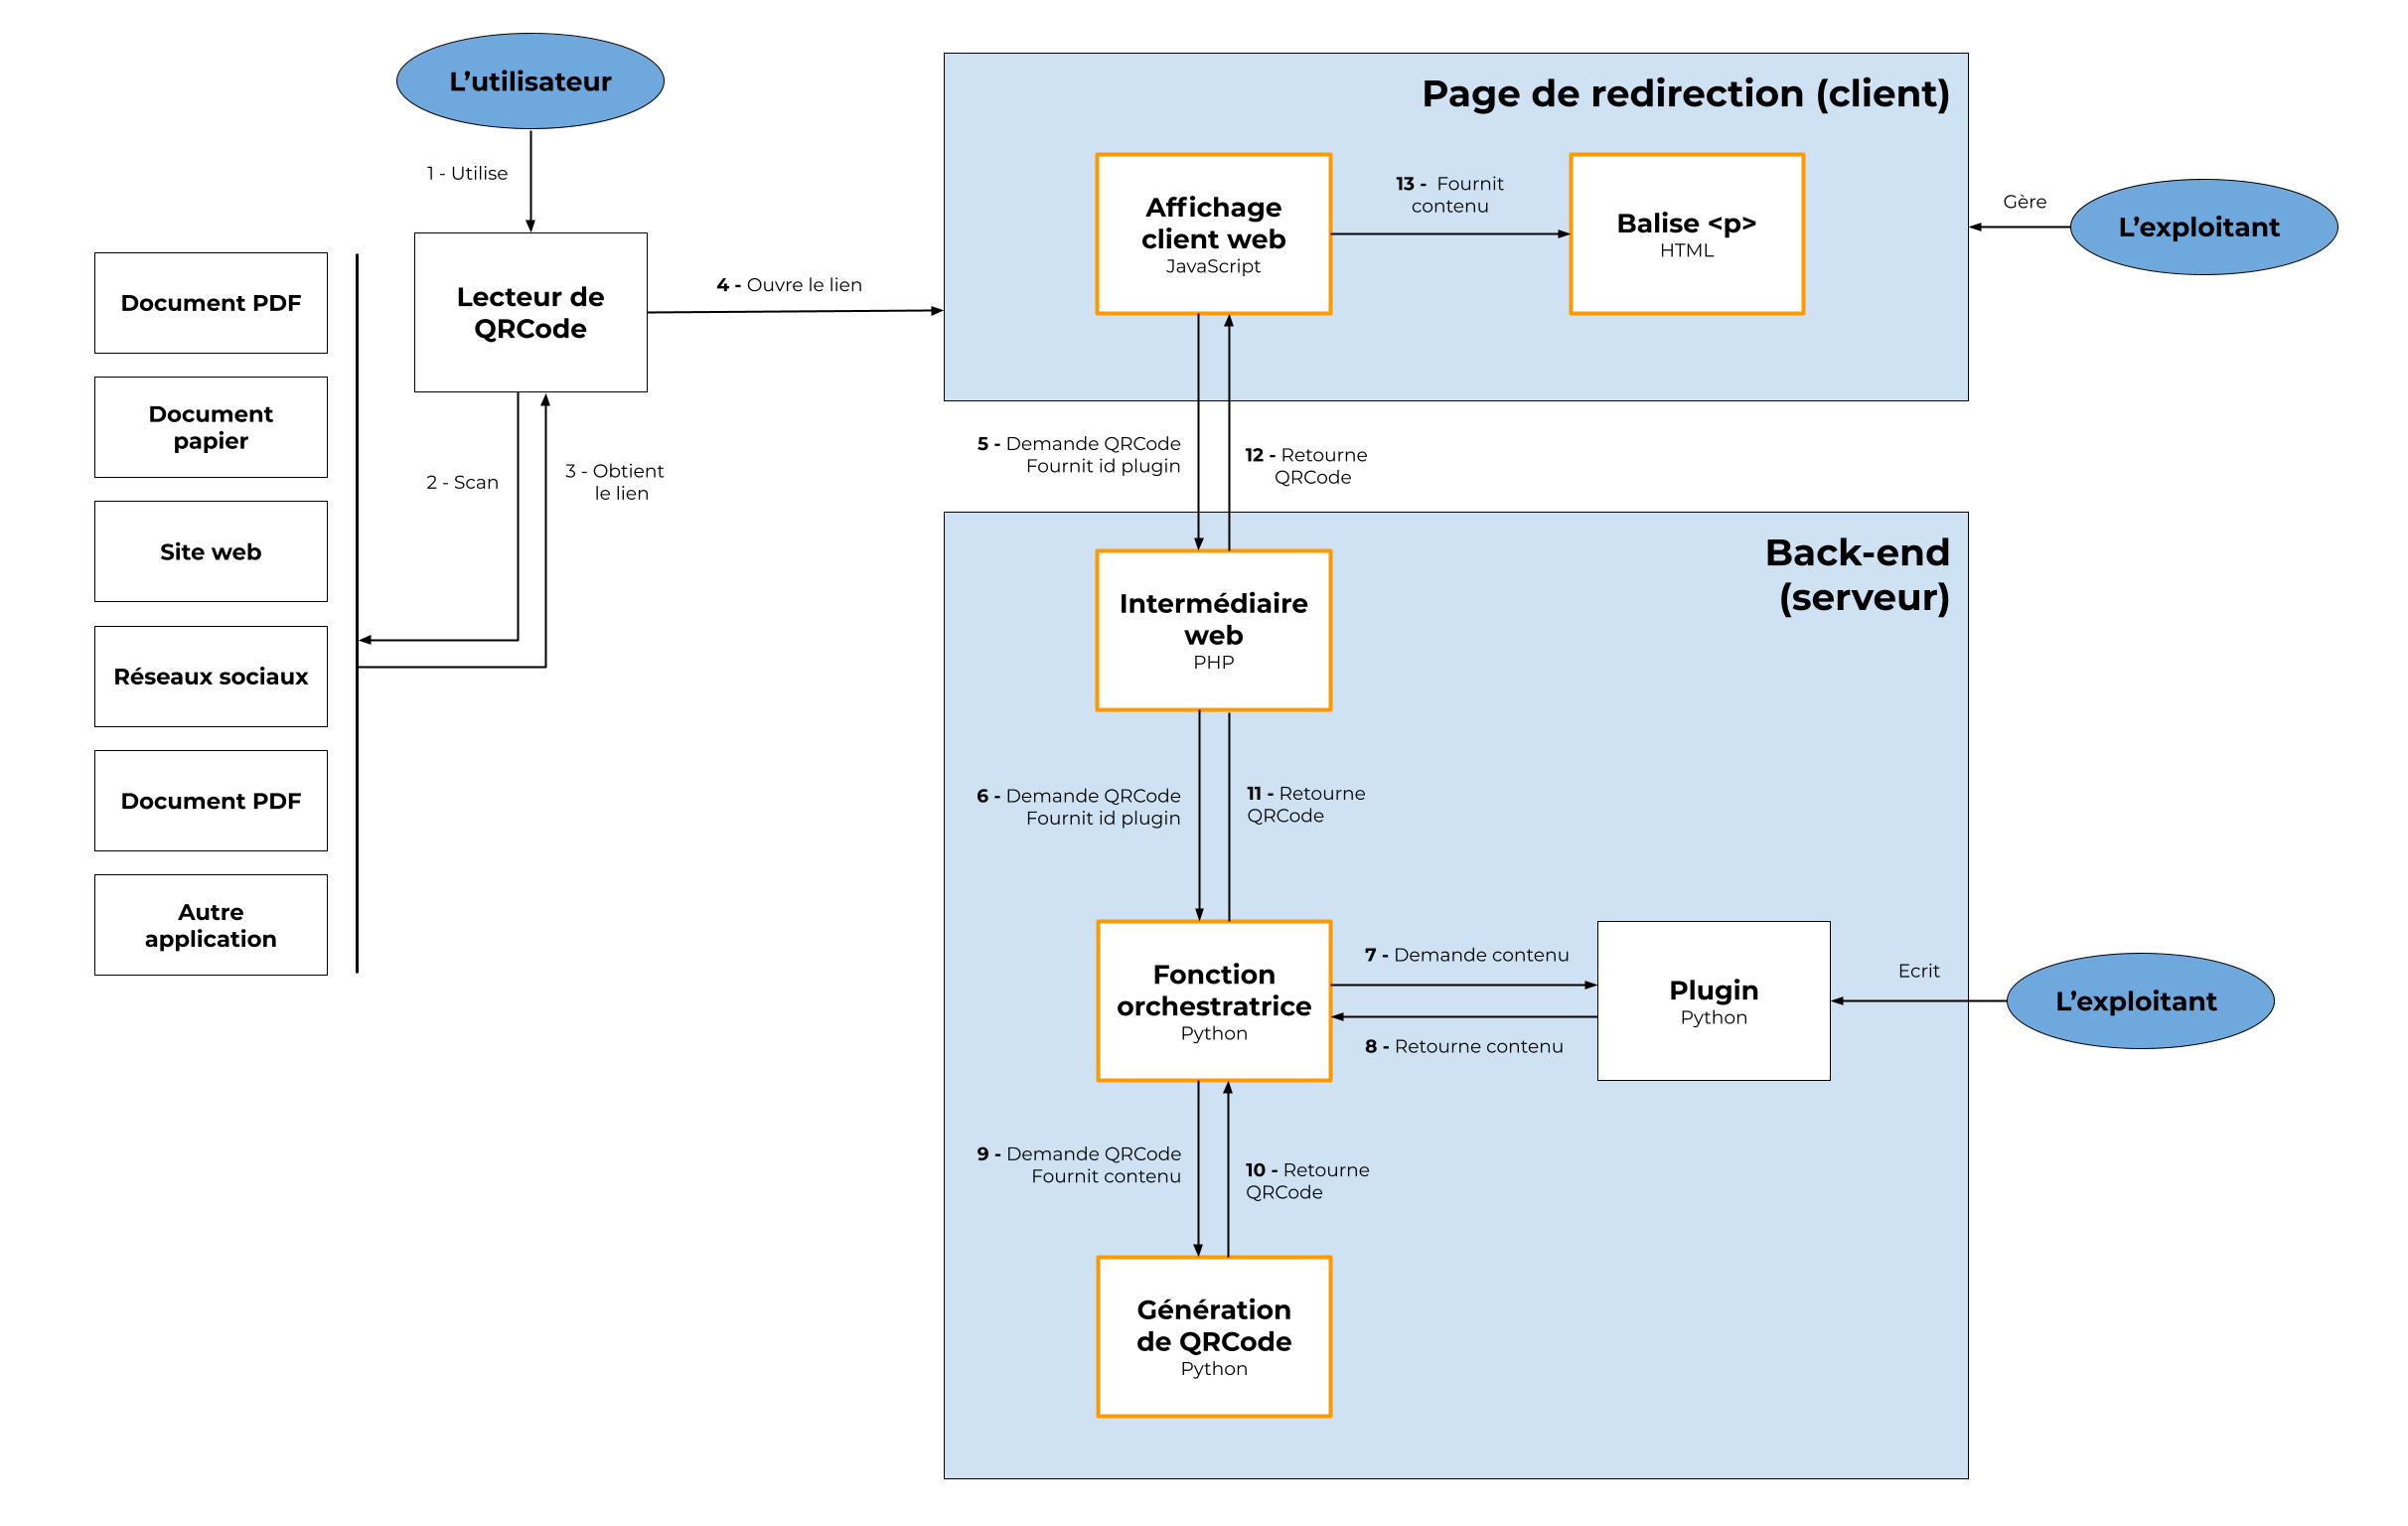
\includegraphics[width=1\textwidth]{Par redirection v2-2.png}
  \caption{Les ellipses bleu foncées sont les acteurs : l'exploitant et l'utilisateur (qui visite la page web). Les rectangles sont les parties du système et ceux entourés en orange sont celles que nous devons coder. C'est-à-dire toutes sauf les plugins qui sont écrits par l'exploitant.}
\end{center}
\end{figure}

\paragraph{Scénario B : scan d'un QR code par un utilisateur}
\begin{itemize}
 \item Un utilisateur trouve un QR code généré par l'exploitant.
 \item Il le scanne, ce qui ouvre un lien web pointant vers la \textbf{page de redirection}.
 \item L'URL possédant également l'ID du QR code, la \textbf{page de redirection} le récupère et fournit l'information à l'\textbf{affichage client web}. 
 \item A partir de là, toutes les opérations suivantes sont les mêmes que pour l'approche par dynamisme intégré, à l'exception de cette dernière étape :
 \item L'\textbf{affichage client web} obtient le QR code (ainsi qu'un fichier JSON possédant des informations notamment le contenu du QR code) et affiche son contenu dans la balise <p> de la \textbf{page de redirection}.
\end{itemize}

\subsubsection{Comparaison des deux approches}
\label{compApproches}

\noindent Voici ci-dessous un tableau pour présenter les principales différences entre les deux approches :\\

    \noindent\begin{longtable}{ | m{.475\textwidth} | m{.475\textwidth} | } 
    \hline
    \textbf{Dynamisme intégré} & \textbf{Dynamisme par redirection} \\ 
    \hline
    Le dynamisme a lieu au niveau de l’affichage du QR code. Le QR code affiché change périodiquement. & Le QR code est statique et renvoie vers un serveur de redirection web. Le dynamisme a lieu au niveau de cette page de redirection.\\
    \hline
    Le QR code ne peut être affiché que sur une interface qui a été prévu pour : le(s) site(s) web de l'exploitant tournant sous PHP et l'afficheur standalone. Un travail de développement doit être effectué pour chaque nouveau système sur lequel le QR code doit être intégré. & Le QR code est statique, il peut donc être exporté, inclus dans un document, imprimé, publié sur n'importe quel site : ce n'est qu'une image. Pas besoin de créer un afficheur standalone.\\
    \hline
    L'intégration d'un QR code dynamique sur un site web nécessite que le système et le serveur web soit sur la même machine. Il faut également inclure un fichier PHP accessible depuis internet, ainsi qu'un script JavaScript sur chaque page possédant un QR code. & Le système est complètement séparé de tout autre système (un serveur web PHP est tout de même nécessaire mais il n'a pas de rapport avec le serveur web du site sur lequel le QR code est déposé).\\
    \hline
    Le contenu est limité à 3,9 Ko (peut être contourné en utilisant un lien web). & Le contenu n'étant pas sur le QR code, il n'y a pas de limite fixe sur la taille du contenu. Cela pourrait être une vidéo de 1.6 Go par exemple, un livre, un jeu...\\
    \hline
    Vis-à-vis des QR codes limités dans le temps (le contenu devient inaccessible à un horodatage spécifié), le contenu dont on souhaite contrôler l'accès se trouvant dans le QR code, n'importe qui peut le copier, le prendre en photo, le publier ailleurs. Il est donc très facile de contourner ce système. & Le contenu dont on souhaite contrôler l'accès étant sur la page web de destination du QR code, l'exploitant a un contrôle totale sur la disponibilité de cette page. Il peut à chaque instant la bloquer, ou la débloquer à souhait.\\
    \hline
    Il n'est pas possible de mettre un mot de passe pour l'accès à l'information. & La page pourrait demander à l'utilisateur d'entrer un mot de passe pour accéder à l'information.\\
    \hline
    Un nouveau QR code doit être généré à chaque changement de son contenu. & Un seul QR code est généré.\\
    \hline
    Il n'est pas possible de savoir par qui, quand et où le QR code a été scanné. & Il serait possible de connaître les adresses IP, l'heure et la position (si on imprime plusieurs QR code à différents endroits d'un bâtiment par exemple) des personnes scannant le QR code. On pourrait également noter les informations du client web comme l'OS, la version du navigateur, la résolution de l'écran...\\
    \hline
    Pas besoin de serveur web pour l'affichage standalone & Nécessite un serveur web quelque soit l'utilisation \\ 
    \hline
    L'utilisateur qui scanne n'a pas besoin d'un accès internet pour accéder au contenu (sauf si il s'agit d'un lien web). &  L'utilisateur doit avoir un accès internet (ou au moins une connexion au réseau local sur lequel tourne le serveur web).\\ 
    \hline
    Aucune charge réseau pour l'affichage standalone, charge réseau supérieur pour l'utilisation web car l'image du QR code est plus lourde que son contenu seul. & Charge réseau proportionelle au nombre d'utilisateurs.\\
    \hline
    \end{longtable}

\bigskip
\newpage
\noindent L'approche par redirection n'était pas dans le cadre initial du projet car elle requiert une installation plus lourde (hébergement d'un service web, ouverture de port, potentielle utilisation de bases de données...). Mais après présentation de la première release et validation de la version par redirection (en plus de la version classique) par notre client, nous l'avons développée. Comme vu dans le tableau comparatif ci-dessus, l'installation, l'utilisation et surtout l'intégration des QR codes sont fortement simplifiées. De manière générale, les deux approches sont compatibles avec les besoins fonctionnels imposés par le client, mais chacune possède des avantages et inconvénients. L'inconvénient majeur du système par redirection est que l'utilisateur final doit avoir un accès internet.\\


\section{Architecture et implémentation}
%Ici on rentre dans le détail du code, avec des décompositions modulaires des classes, le fonctionnement du code (diagrammes séquentiels, etc..) et les différents blocs qui composent notre archi (front, back).\\
\noindent Voici une représentation de l'architecture complète de notre projet sous forme de diagramme UML :\\
\noindent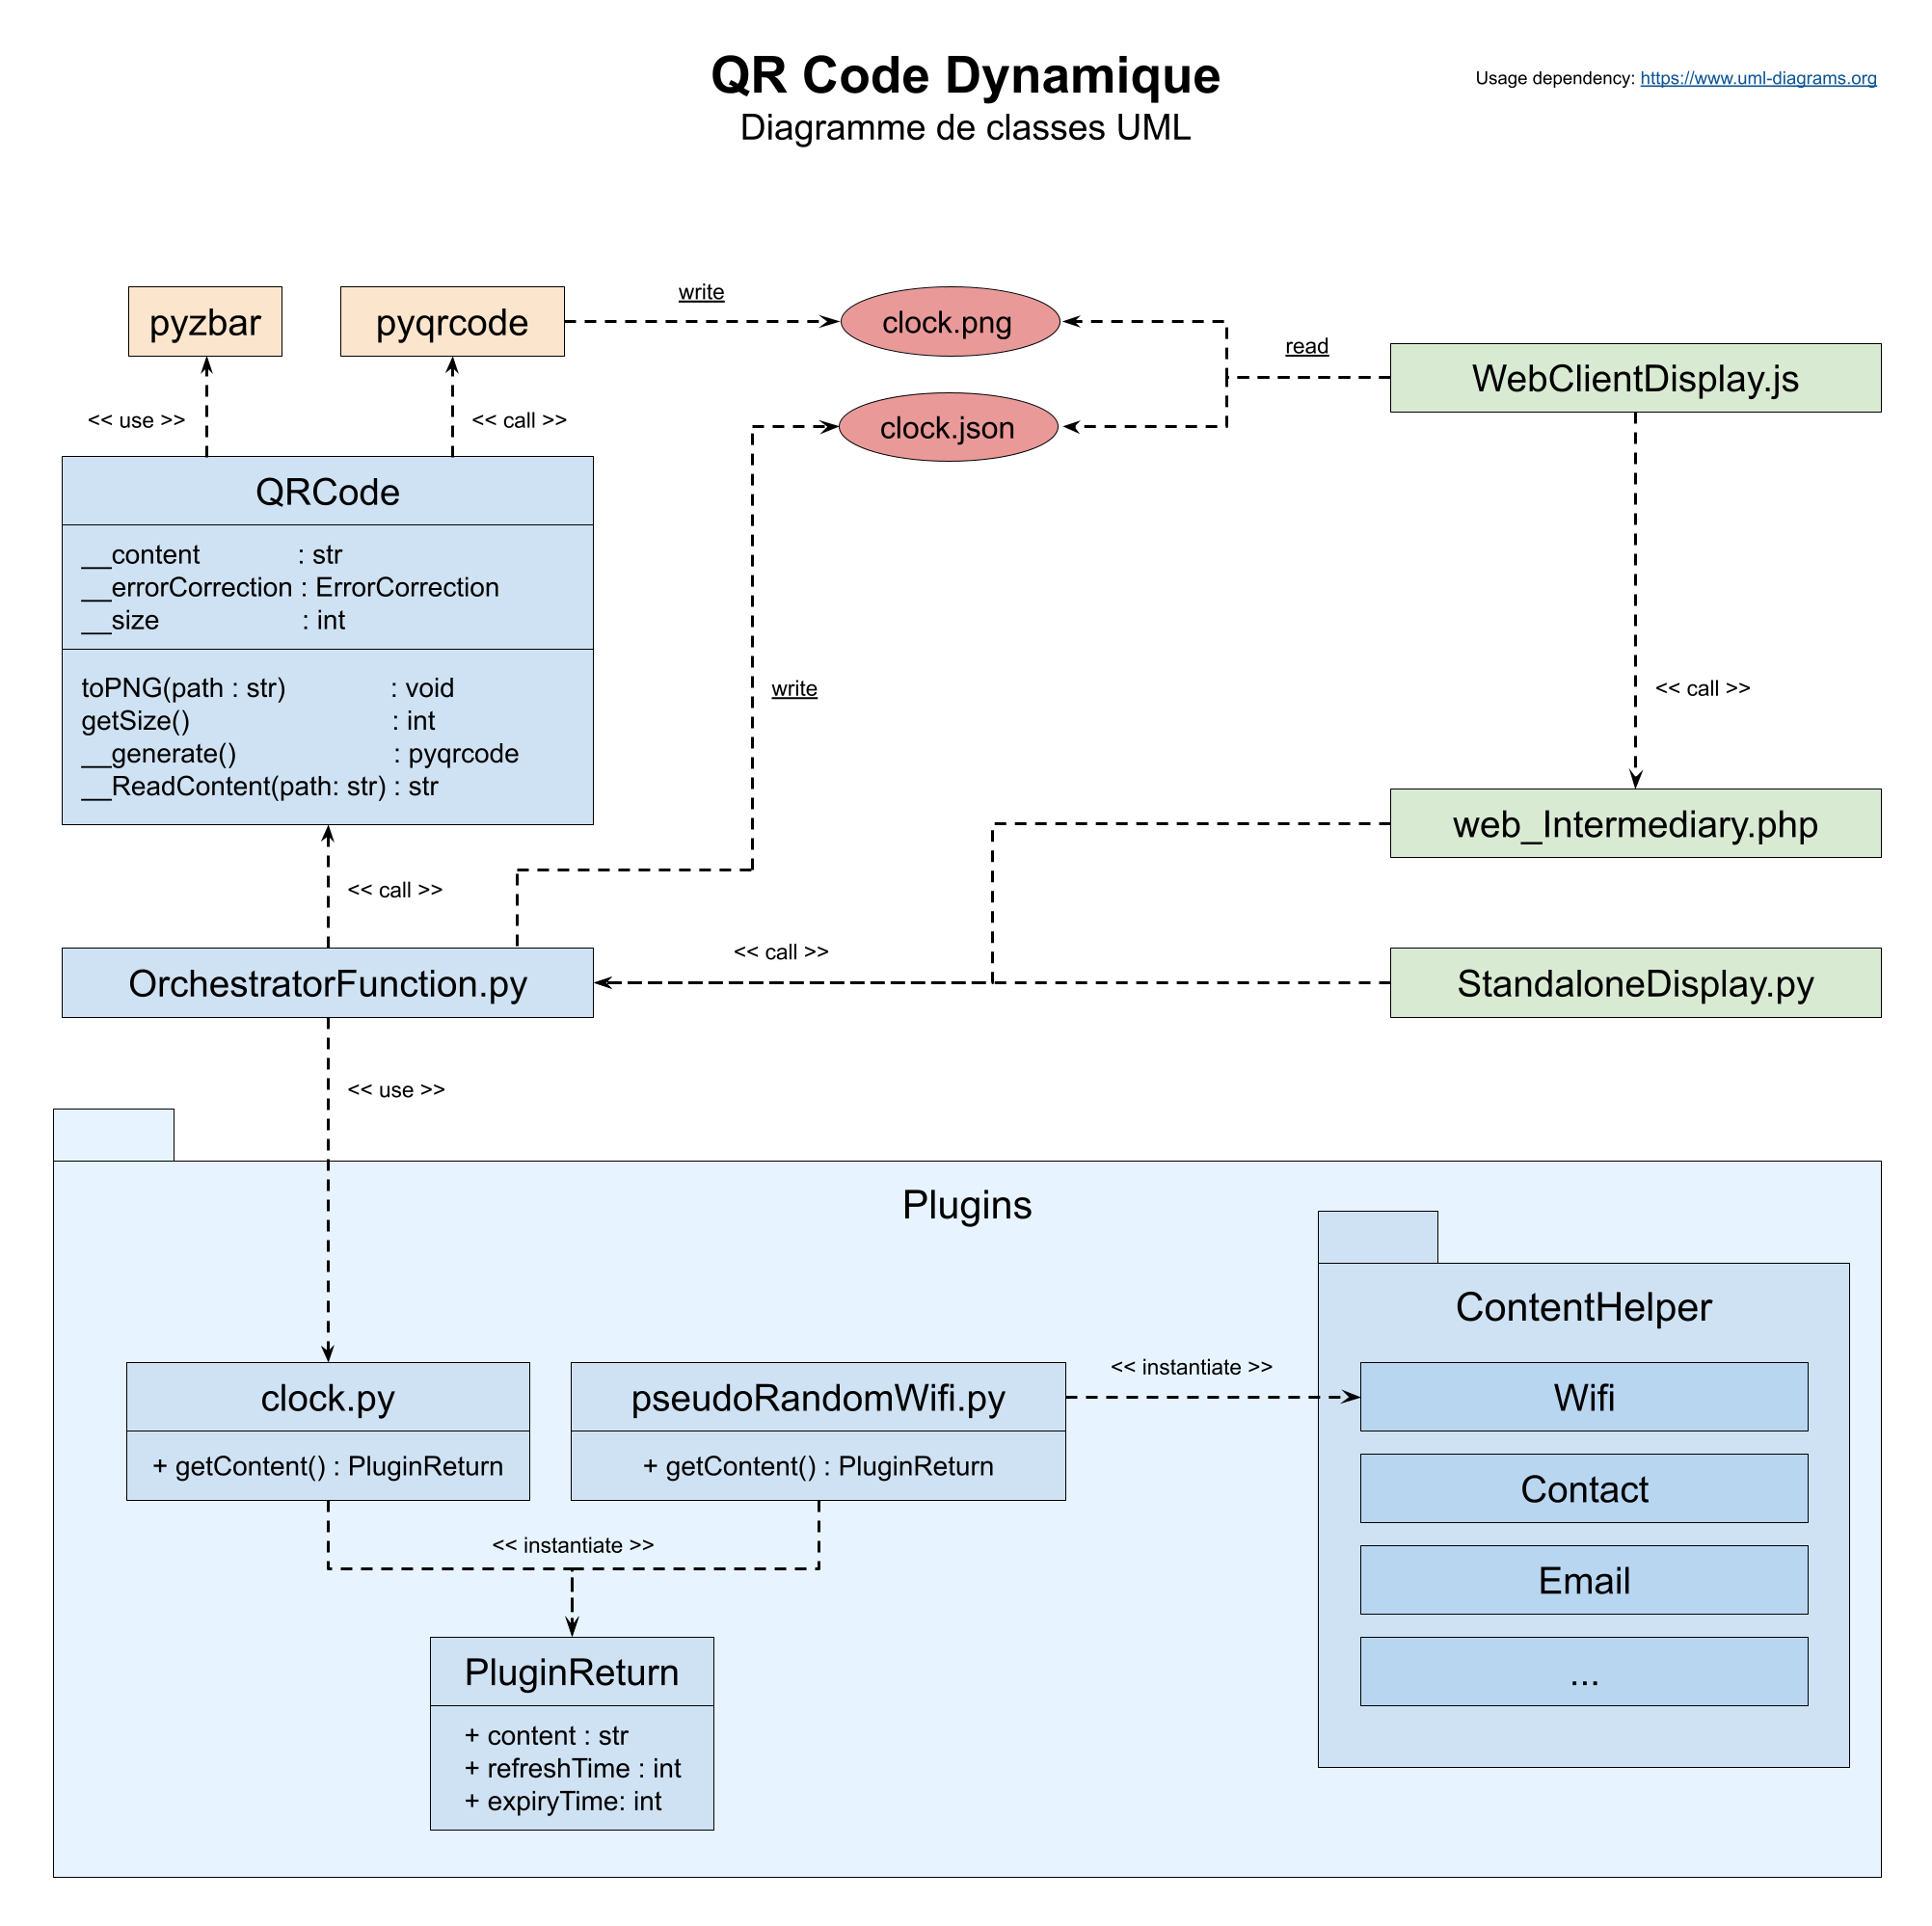
\includegraphics[width=\textwidth]{UML Class.png} %!TODO! Tout en anglais

% BOF! ici faut expliquer le diagramme UML comme pendant l'audit 
% -> je suis pas sûr de ce que j'ai écrit.
\noindent On peut voir ici la manière dont est découpé notre projet. Nous avons choisi de le diviser en deux blocs principaux : le BackEnd en bleu, le FrontEnd en vert. Les bibliothèques d'encodage/décodage de QR code font partie du bloc BackEnd et sont en orange. Le détail de chaque élément des différents blocs principaux sera donné plus bas. Ici, le diagramme présente le cas d'utilisation d'un plugin nommé clock.py, mais n'importe quel autre nom de plugin aurait fonctionné de la même manière.\\

\noindent Voici un diagramme séquentiel montrant une situation de fonctionnement de notre programme, à savoir la demande de génération d'un QR code par l'afficheur, et la décomposition des échanges qui suivent entre les parties du programme :\\
\noindent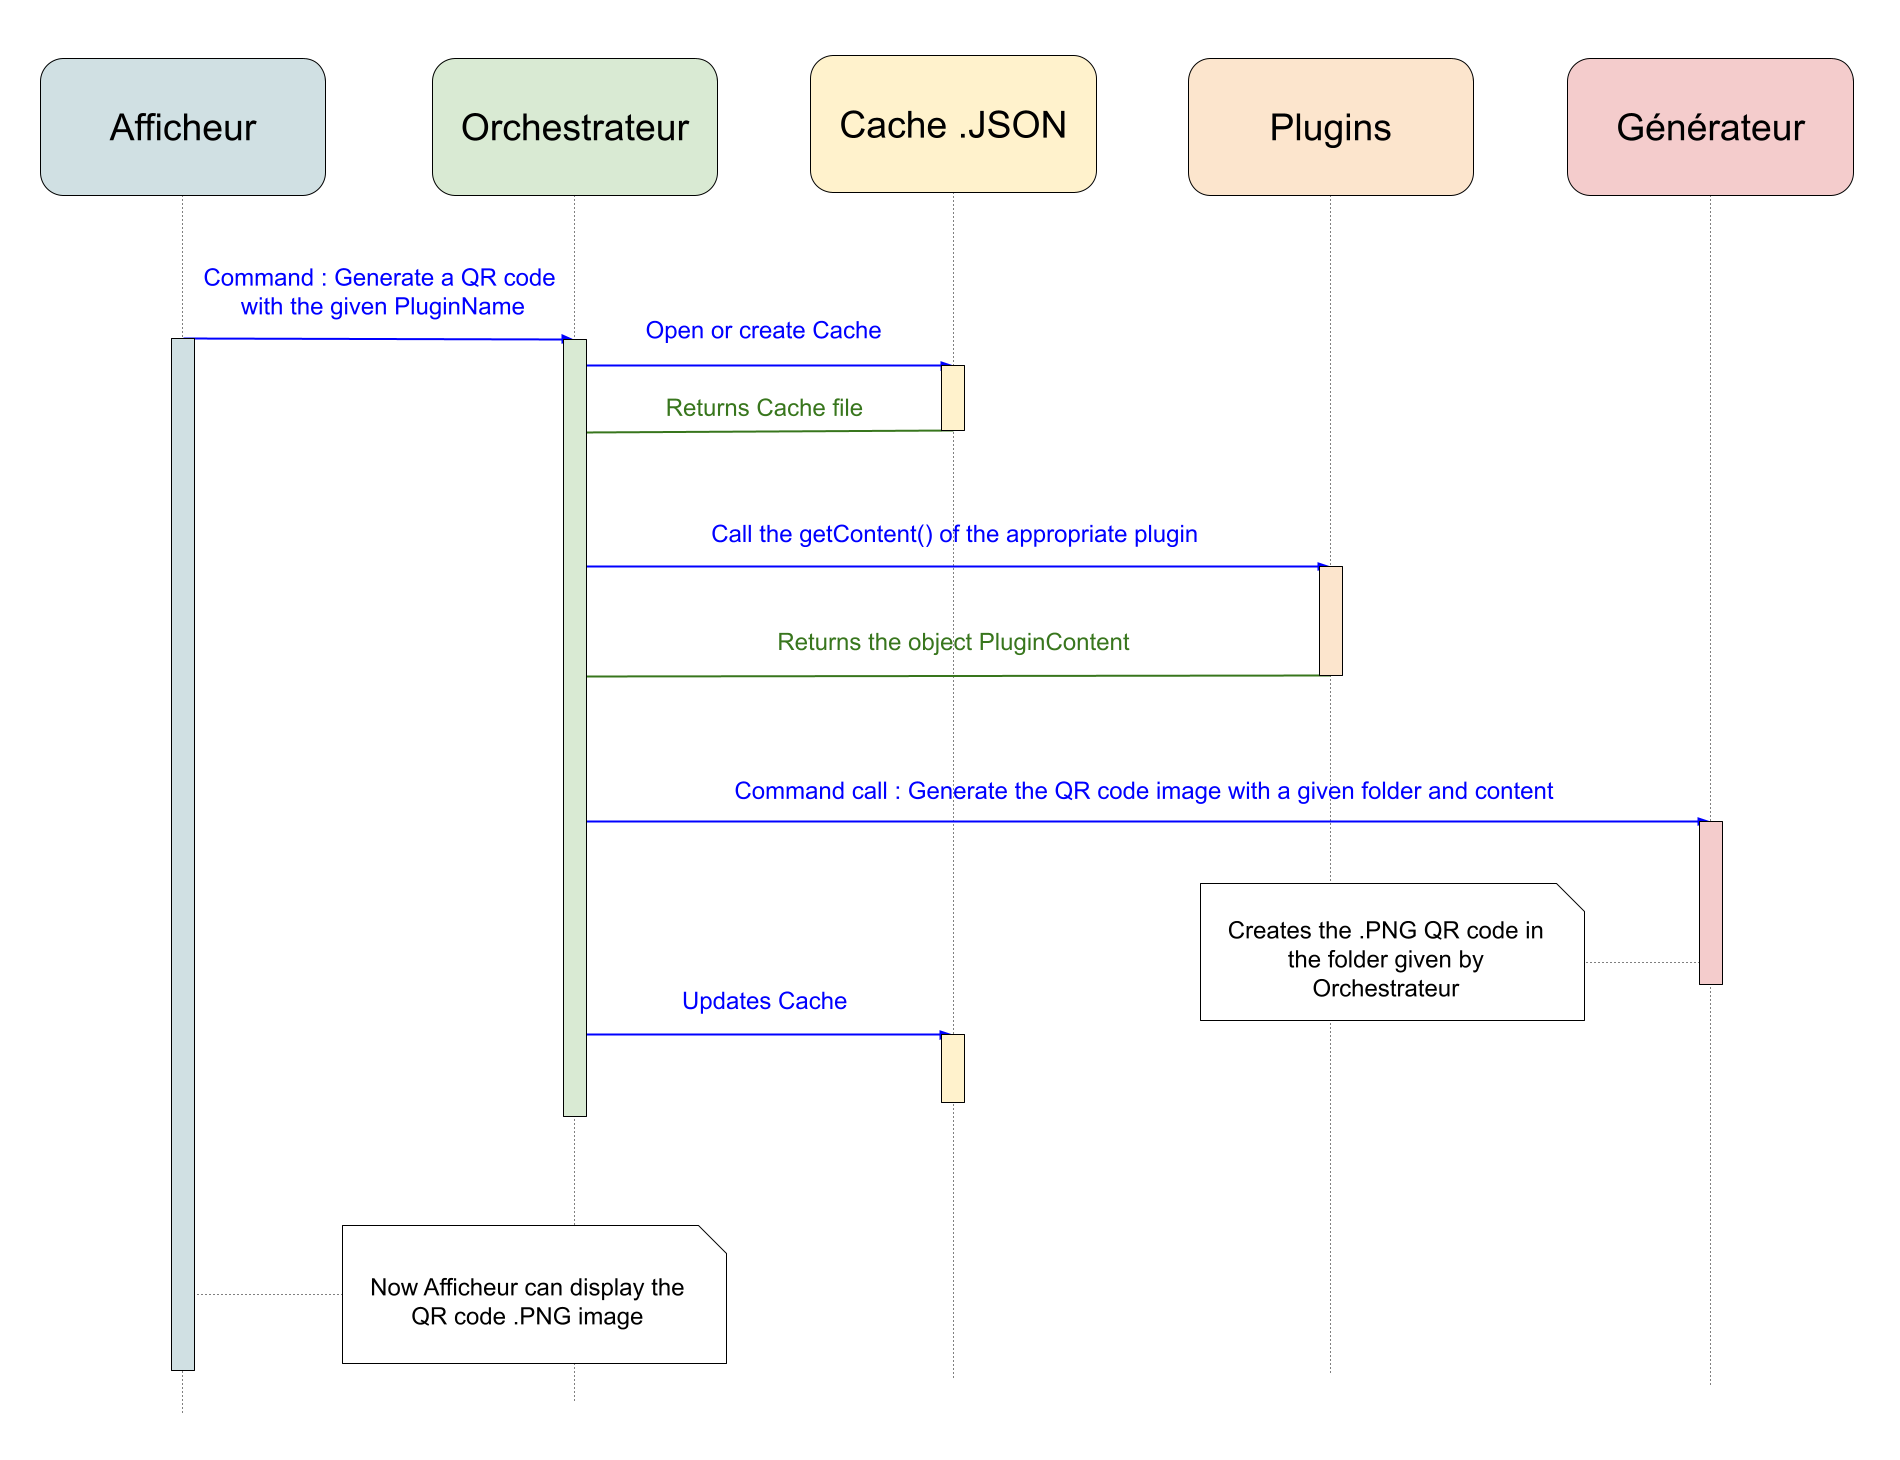
\includegraphics[width=\textwidth]{diag_seq.png} 
Ce diagramme séquentiel permet de donner une approche visuelle simpliste d'une situation entraînant des dialogues entre les différentes partie de notre programme.\\

\noindent Nous avons également fait passer des tests avec la bibliothèque pycodestyle \footnote{\url{https://pypi.org/project/pycodestyle/}, (consulté le 09-04-2021)}, un linter qui nous garantit que notre code est à la norme PEP 8\footnote{\url{https://www.python.org/dev/peps/pep-0008/}, (consulté le 09-04-2021)}.

\newpage
\subsection{BackEnd}
\label{backend}

\begin{itemize}
 \item 
     \textbf{Fonction orchestratrice (Programme CLI)} : la fonction orchestratrice est l'unique point d'entrée de la partie backEnd. Le programme possède une "Interface en ligne de commande" (CLI). Voila la structure d'une commande : 
     
     \verb|python OrchestratorFunction.py <nom du plugin> <dossier de destination>|. 
     
     Le but est de prendre en paramètre un nom de plugin et un dossier de destination, puis de générer un QR code dans le dossier de destination ayant pour contenu la chaîne de caractères fournie par le plugin correspondant.
\noindent De manière un peu plus détaillée, voici les étapes de l'exécution de la Fonction orchestratrice :
    \begin{enumerate}
        \item Importe le plugin dont le nom est donné en paramètre.
        \item Fait un appel à la fonction getContent qui est présente dans chaque plugin.
        \item Cette fonction retourne un objet de type PluginReturn.
        \item L'attribut contenu de cet objet de retour est passé à la partie "Génération de QR code" (un objet de classe QRCode).
        \item Le dossier de destination donnée en paramètre est également fourni à l'objet QRCode lors de l'appel de sa méthode toPNG.
        \item Le QR code possédant le contenu fourni par le plugin est maintenant généré dans le dossier de destination.
    \end{enumerate}
        
 \item 
    \textbf{Génération QR code (Class)} : la classe QRCode fournit une version simplifiée de la bibliothèque Pyqrcode, se focalisant uniquement sur les aspects nécessaires pour ce projet (il s'agit du patron de conception Façade). Lors de la construction d'un objet QRCode, différents paramètres peuvent/doivent être fournis : 
    \begin{itemize}
        \item (Obligatoire) le contenu du QR code (une chaîne de caractères).
        \item (Optionnel) le niveau de correction du QR code (par défaut niveau médium).
        \item (Optionnel) la taille du QR code (par défaut la taille la plus petite possible est sélectionnée).
    \end{itemize}
    
    Un objet de classe QRCode possède également la méthode toPNG qui permet d'exporter le QR code sous format PNG dans un dossier de destination fourni en paramètre.
    \\
 
 \item \textbf{Plugins (Package)} : le dossier et package "Plugins" contient les plugins écrits par l'exploitant mais également d'autres classes permettant de simplifier la création de QR codes complexes (connexion WiFi, envoi de mail...).
 
 % TODO! Pas totalement fini
    \begin{itemize}
        \item \textbf{Plugin (Fonction)} : voici un exemple de plugin appelé "clock" :\\
    
        \begin{lstlisting}
from PluginReturn.PluginReturn import PluginReturn
import time

def getContent() -> PluginReturn:
    content = time.time()
    refreshTime = 5  # in s
    return PluginReturn(content, refreshTime)
        \end{lstlisting}
        
        On peut voir ici qu'on définit le contenu comme étant la date et heure actuelle, et le temps de rafraîchissement est fixé à 5 secondes. La fonction doit toujours retourner un objet de type PluginReturn.\\
    
        \item \textbf{ContentHelper (Package)} : lorsqu'un QR code est scanné, son contenu peut être interprété de différentes manières suivant la structure de son contenu. Le "type" par défaut est "Texte" (pas de structure particulière). Il existe également "URL" (le contenu commence par http:// ou https://), ou "Téléphone" (le contenu commence par tel:). D'autres types ont été définis dans la partie \ref{stadardQR}. L'objectif du package ContentHelper est de fournir des "formulaires" simplifiés pour la génération de contenu typé.
        
        Par exemple, si l'exploitant souhaite générer des QR codes qui permettent la connexion à un réseau WiFi, il peut utiliser la classe ContentHelper.Wifi.
        Il suffit pour cela d'utiliser le constructeur de cette classe : 
        
        \verb|content = Wifi('Livebox-0123', WifiTypes.wpa, 'Mon super mot de passe')|.
        
        Lorsque l'objet Wifi sera converti en chaîne de caractères, voici le résultat qui sera obtenu :
        
        \verb|WIFI:T:WPA;S:Livebox-0123;P:Mon super mot de passe|.\\
        
        \item \textbf{PluginReturn (Class)} : l'objet qui est retourné par les plugins et qui est utilisé par la fonction orchestractice pour la génération du QR code. Il y a trois paramètres : 
        \begin{itemize}
            \item content (Obligatoire) le contenu du QR code (une chaîne de caractères).
            \item refreshTime (Optionnel) la durée pendant laquelle on considère le contenu du QR code comme valide. Ex: si refreshTime vaut 60, l'image de QR code sera conservé pendant au moins 60 secondes. Par défaut, il est infini, le QR code est statique.
            \item expiryTime (Optionnel) l'horodatage (de type datetime) déterminant quand le contenu du QR code deviendra inaccessible. Par défaut il est infini.
        \end{itemize}
        
        Il est important de noter que la valeur refreshTime est à choisir avec précaution. La fonction orchestratrice stocke cette valeur dans un fichier JSON et elle l'utilise pour limiter le nombre d'appels au plugin (qui peut être une opération coûteuse suivant son fonctionnement). Si la période formée par le refreshTime n'est pas révolue, tout appel vers le backEnd sera inutile. C'est pour cela que cette valeur est également transmise aux clients web et standalone pour limiter le nombre d'appels qu'ils font vers le backEnd.
        
        C'est donc un système qui pourrait s'apparenter aux TTL des serveurs DNS : si l'on souhaite changer n'importe quelle propriété d'un plugin, il y a une durée de propagation qui est inférieur ou égale au refreshTime. Ce détail est également important pour les QR codes limités dans le temps (possédant un expiryTime) : si le refreshTime est égal à 24h, alors il est possible que les clients puissent accéder au contenu du QR code même 24 heures après l'horodatage défini par l'expiryTime.\\
        
    \end{itemize}
\end{itemize}


\subsection{FrontEnd}
\label{frontend}

\noindent Pour la partie FrontEnd, on dispose de deux afficheurs différents :\\
La version Standalone en Python, et la version Web en Html/Css/Js.\\
Les deux afficheurs fonctionnent sur le même principe, à savoir demander la génération d'un QR code selon le plugin associé, et rafraîchir l'image de QR code affichée à l'écran de manière régulière.

\subsubsection{Standalone}
\noindent Cette commande permet d'exécuter le programme : python StandaloneDisplay.py.\\
L'afficheur utilise la librairie tkinter pour l'interface utilisateur. Elle permet une compatibilité entre Linux, Windows et d'autre système comme le Raspberry.\\
Le but est de proposer à l'utilisateur une interface lui permettant de sélectionner un plugin à utiliser, et ensuite de demander la génération de l'image de QR code à la fonction orchestratrice, le récupérer dans le dossier qrcodes/<PluginName>.png et l'afficher dans la fenêtre d'environnement tkinter. Le rafraîchissement de l'image doit également être géré automatiquement.\\

\noindent Il est possible de choisir le QR Code à afficher selon les plugins disponibles dans le menu déroulant, ainsi que de passer de la version QR code dynamique à redirection à l'aide d'une checkbox.
L'afficheur gère également des caches en .json stockés dans le dossier qrcodes/<PluginName>.json permettant de limiter le nombre d'appels à l'orchestratrice.\\

Voici un détail des étapes de l'exécution de l'afficheur :
\begin{enumerate}
\item Initialisation de la fenêtre tkinter qui s'adapte aux dimensions de l'écran.
\item Récupération de la liste des plugins disponibles (fonction getPluginsNames) pour les ajouter au menu déroulant.
\item Appel de la fonction updateImage qui va appeler Orchestrator pour générer l'image du QR Code selon le plugin choisi dans la liste, puis calculer grâce au cache le prochain refreshTime, pour savoir quand rappeler la fonction updateImage.
\item Mise à jour du timerText qui affiche à l'écran la date/heure du prochain refresh du QR code.
\item Appel de displayImage pour afficher l'image de QR code générée.\\
\end{enumerate}
Autres fonctions :\\
- userInput : appelée quand on change le plugin dans la liste, ou quand on coche la boite à cocher.\\
- loadJSON : ouvre le fichier de cache .json d'un plugin demandé (selon son filePath).\\

\noindent En fonction de si la checkbox est cochée ou non, le comportement de updateImage diffère.\\
En effet en cas de mode redirection, il n'est plus nécessaire de boucler la fonction car le QR code affiché est statique (pas de refreshTime). Également, il n'est plus nécessaire d'afficher le timerText pour cette image, il sera donc vide.\\

\noindent Nous avons apporté plusieurs extensions à cet afficheur, qui améliore son utilisation par rapport à la version minimale qui n'affichait qu'un QR code sur une fenêtre. On retrouve donc dans ces extensions :

\begin{enumerate}
\item Menu déroulant pour savoir quel QR code afficher selon les plugins disponibles.
\item Boite à cocher permettant d'alterner avec la version par redirection.
\item Affiche de la "date de péremption" d'un QR code, à savoir la date+heure du prochain refresh.
\item L'affichage d'un QR code d'erreur par défaut en cas de problème de génération, de rendu ou d'affichage d'un QR code demandé. 
\end{enumerate}

%look
\noindent Il y a un détail d'implémentation que nous voulions expliquer : il est une duplication de code pour la fonction getPluginsNames() qu'on retrouve à la fois dans OrchestratorFunction.py et StandaloneDisplay.py. Nous n'avons pas souhaité créer un fichier d'outil commun au deux et la raison est la suivante : l'afficheur standalone aurait pu être écrit sous n'importe quelle langage. Si par exemple, StandaloneDisplay avait été écrit en Java, la question ne se serait pas posé.

\subsubsection{Web}
\noindent Afin d'ajouter les capacités d'affichage de QR code dynamique sur un site web, l'exploitant doit héberger un fichier PHP (web\_Intermediary.php), ainsi qu'un fichier Javascript (WebClientDisplay.js). Ce dernier doit être importé à toute page web affichant le QR code. Pour finir, une ligne doit être ajoutée au code HTML de la page à la position où le QR code doit être affiché (ici nous prendrons l'exemple du nom de plugin clock): 
\verb|<div class="qrCodeDyn" pluginName="clock"></div>|.\\
\noindent
\begin{itemize}
\item Une fois que la page est chargée, la fonction WebClientDisplay.js récupère chaque élément ayant comme class "qrCodeDyn".
\item Pour chaque élément récupéré on va faire un appel à web\_Intermediary.php en transmettant également le nom du plugin (ici : web\_Intermediary.php?plugin=clock).
\item Avec cela l'intermédiaire récupère le nom du plugin et fait un appel à la fonction orchestratrice.
\item Le backEnd va générer l'image du QR code ainsi qu'un fichier JSON pour transmettre certaines informations comme la durée de validité ou le contenu du QR code.
\item L'affichage client web va ensuite générer une balise <img> avec pour source l'image générée, lire le fichier JSON et créer un Timeout (une relance de la fonction dans un intervalle donné).\\
\end{itemize}

\noindent Il y a également un détail important : les navigateurs web implémentent tous un système de cache pour les images et autres ressources. Dans notre situation nous voulons pouvoir recharger l'image de QR alors que son URL reste inchangé. Les navigateurs ne permettant pas cette opération, ils vont tout simplement utiliser la version en cache. Afin de leurrer le navigateur, nous ajoutons un paramètre GET lorsque l'affichage client web crée la balise <img>, en apposant l'heure UNIX à la fin de l'URL.

\noindent Comme extension apportée nous avons ajouté la possibilité de cliquer sur l'image du QR code pour faire apparaître un pop-up dans lequel est affiché le contenu du QR code. Ce contenu est récupéré grâce au fichier json tout comme la durée de vie.


\subsection{Systèmes de caches}
\label{systemesCaches}
% BOF! expliquer les fichiers .json + j'ai changé le graphe du cache (mis le nouveau du diapo) donc le texte est pas forcément en lien avec l'image. 

Nous pouvons imaginer qu'un site web accueillant des milliers d'utilisateurs en parallèle n'aurait pas la puissance de calcul nécessaire pour constamment générer des QR codes à la volée (de plus que la majorité du temps, leurs contenus resteront inchangés). Nous avons donc choisi de mettre en place un système de cache pour anticiper certains problèmes de performances.


\begin{figure}[H]
    \centering
    %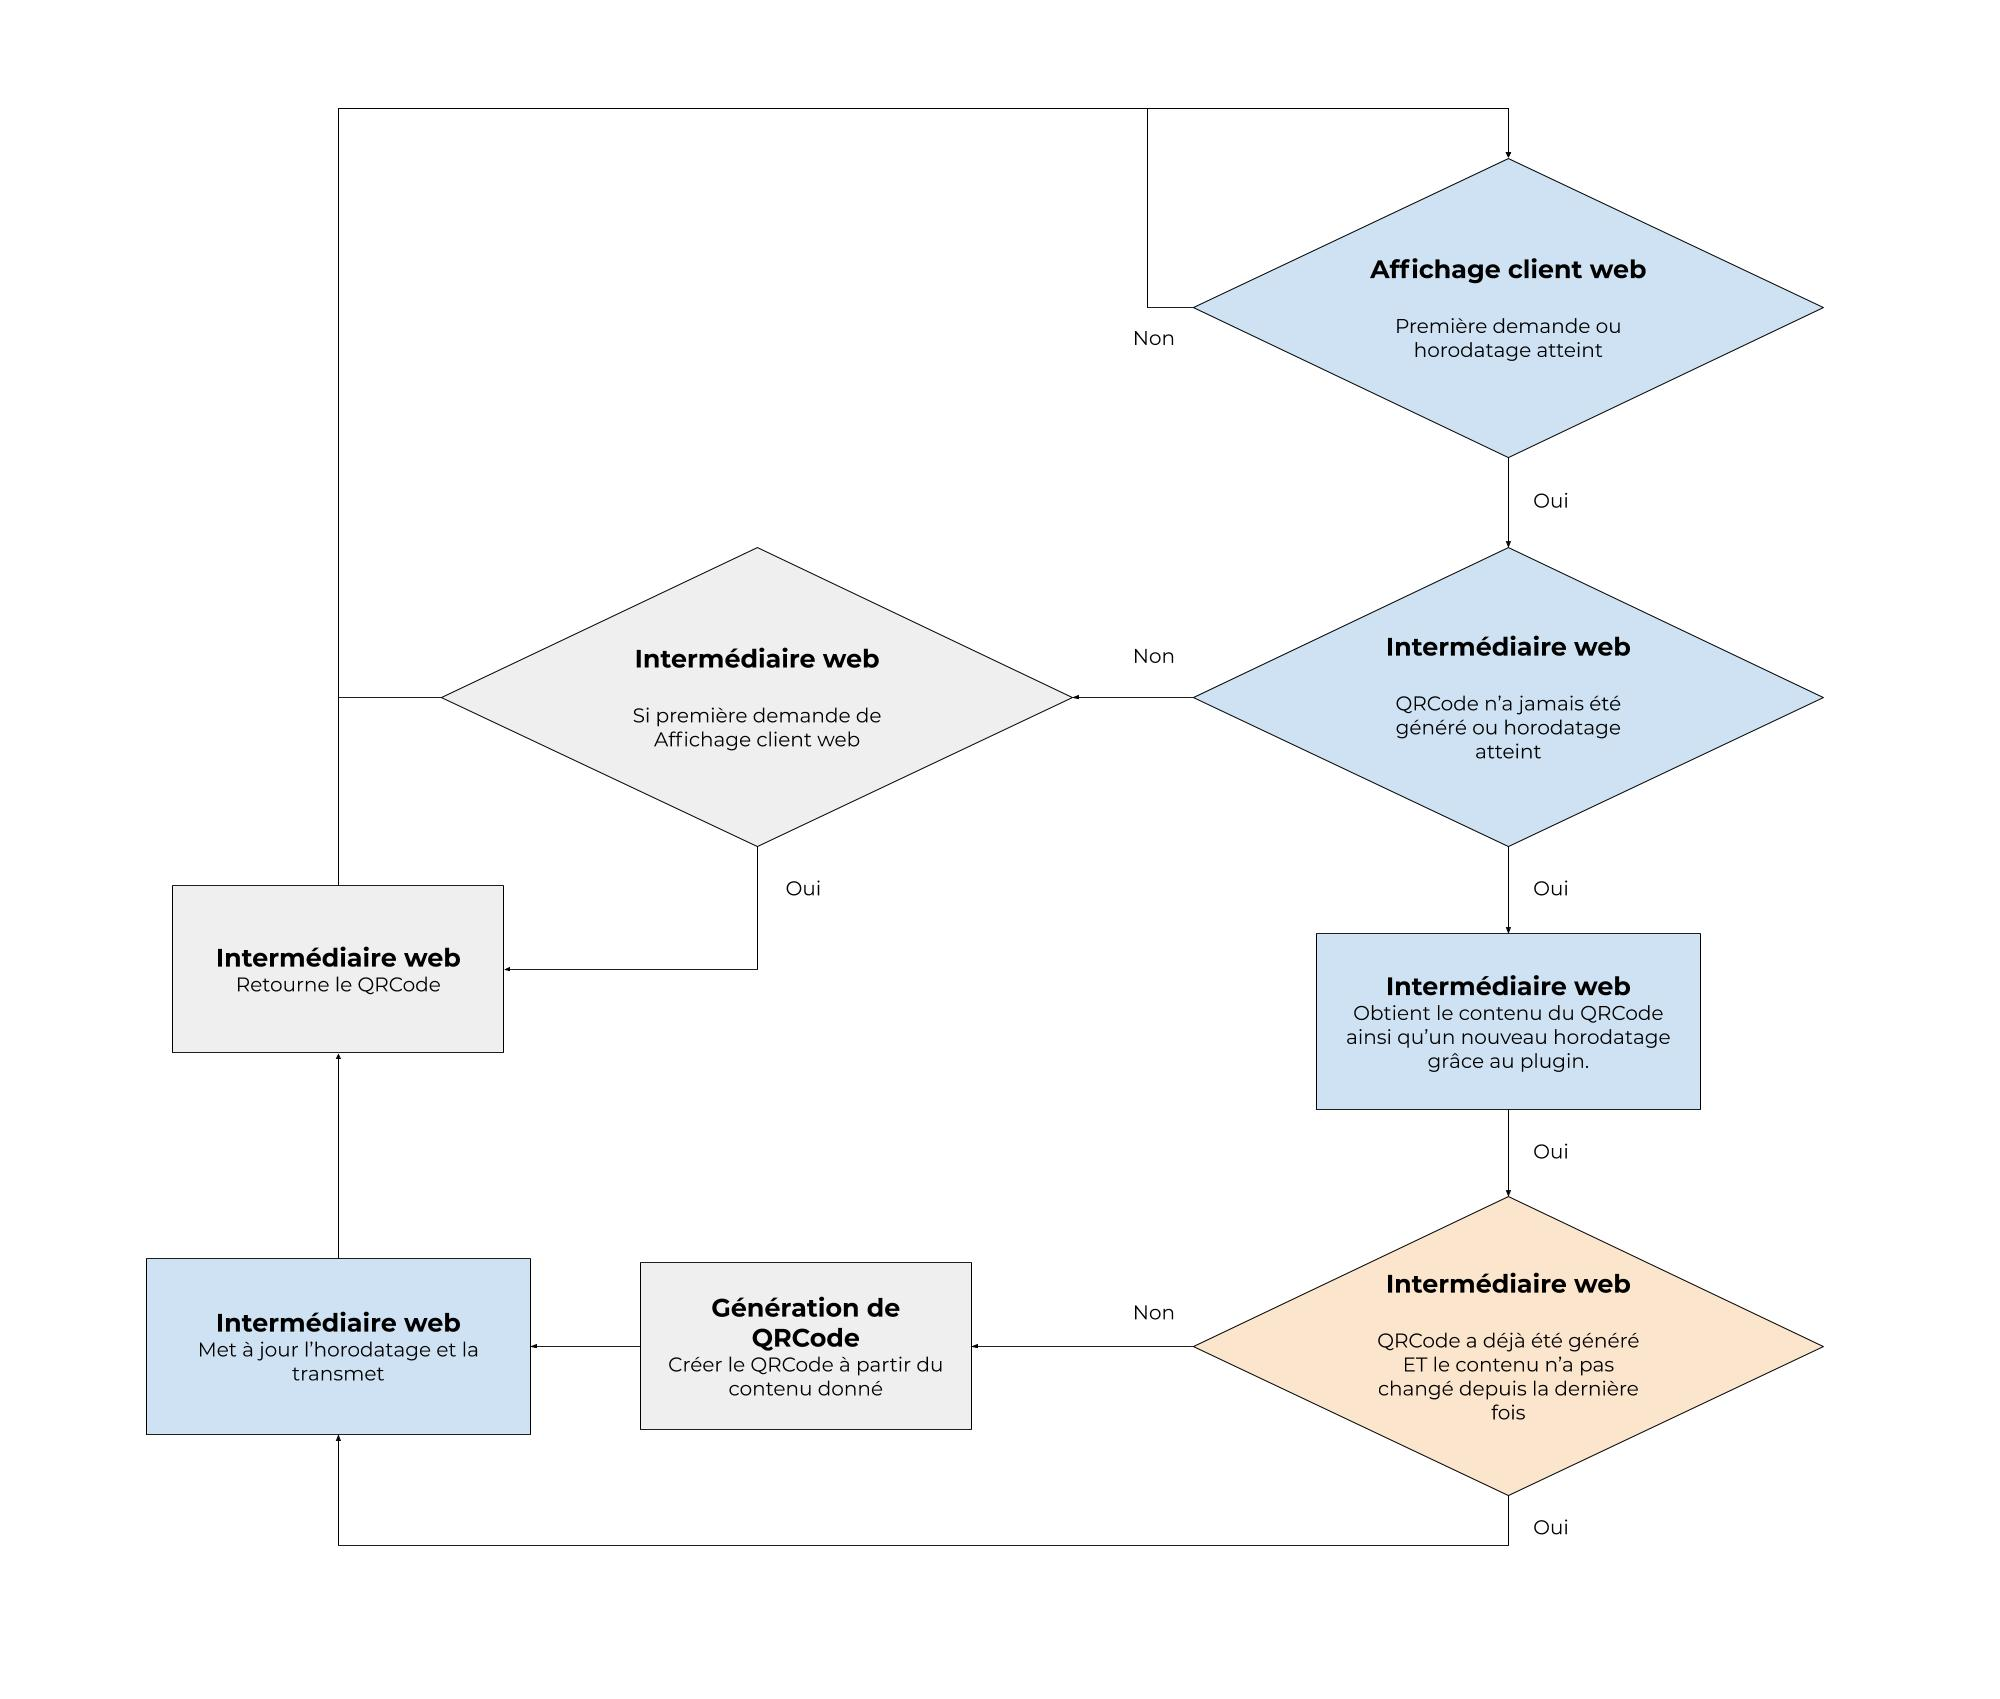
\includegraphics[width=.8\textwidth]{Logique cache.jpg}
    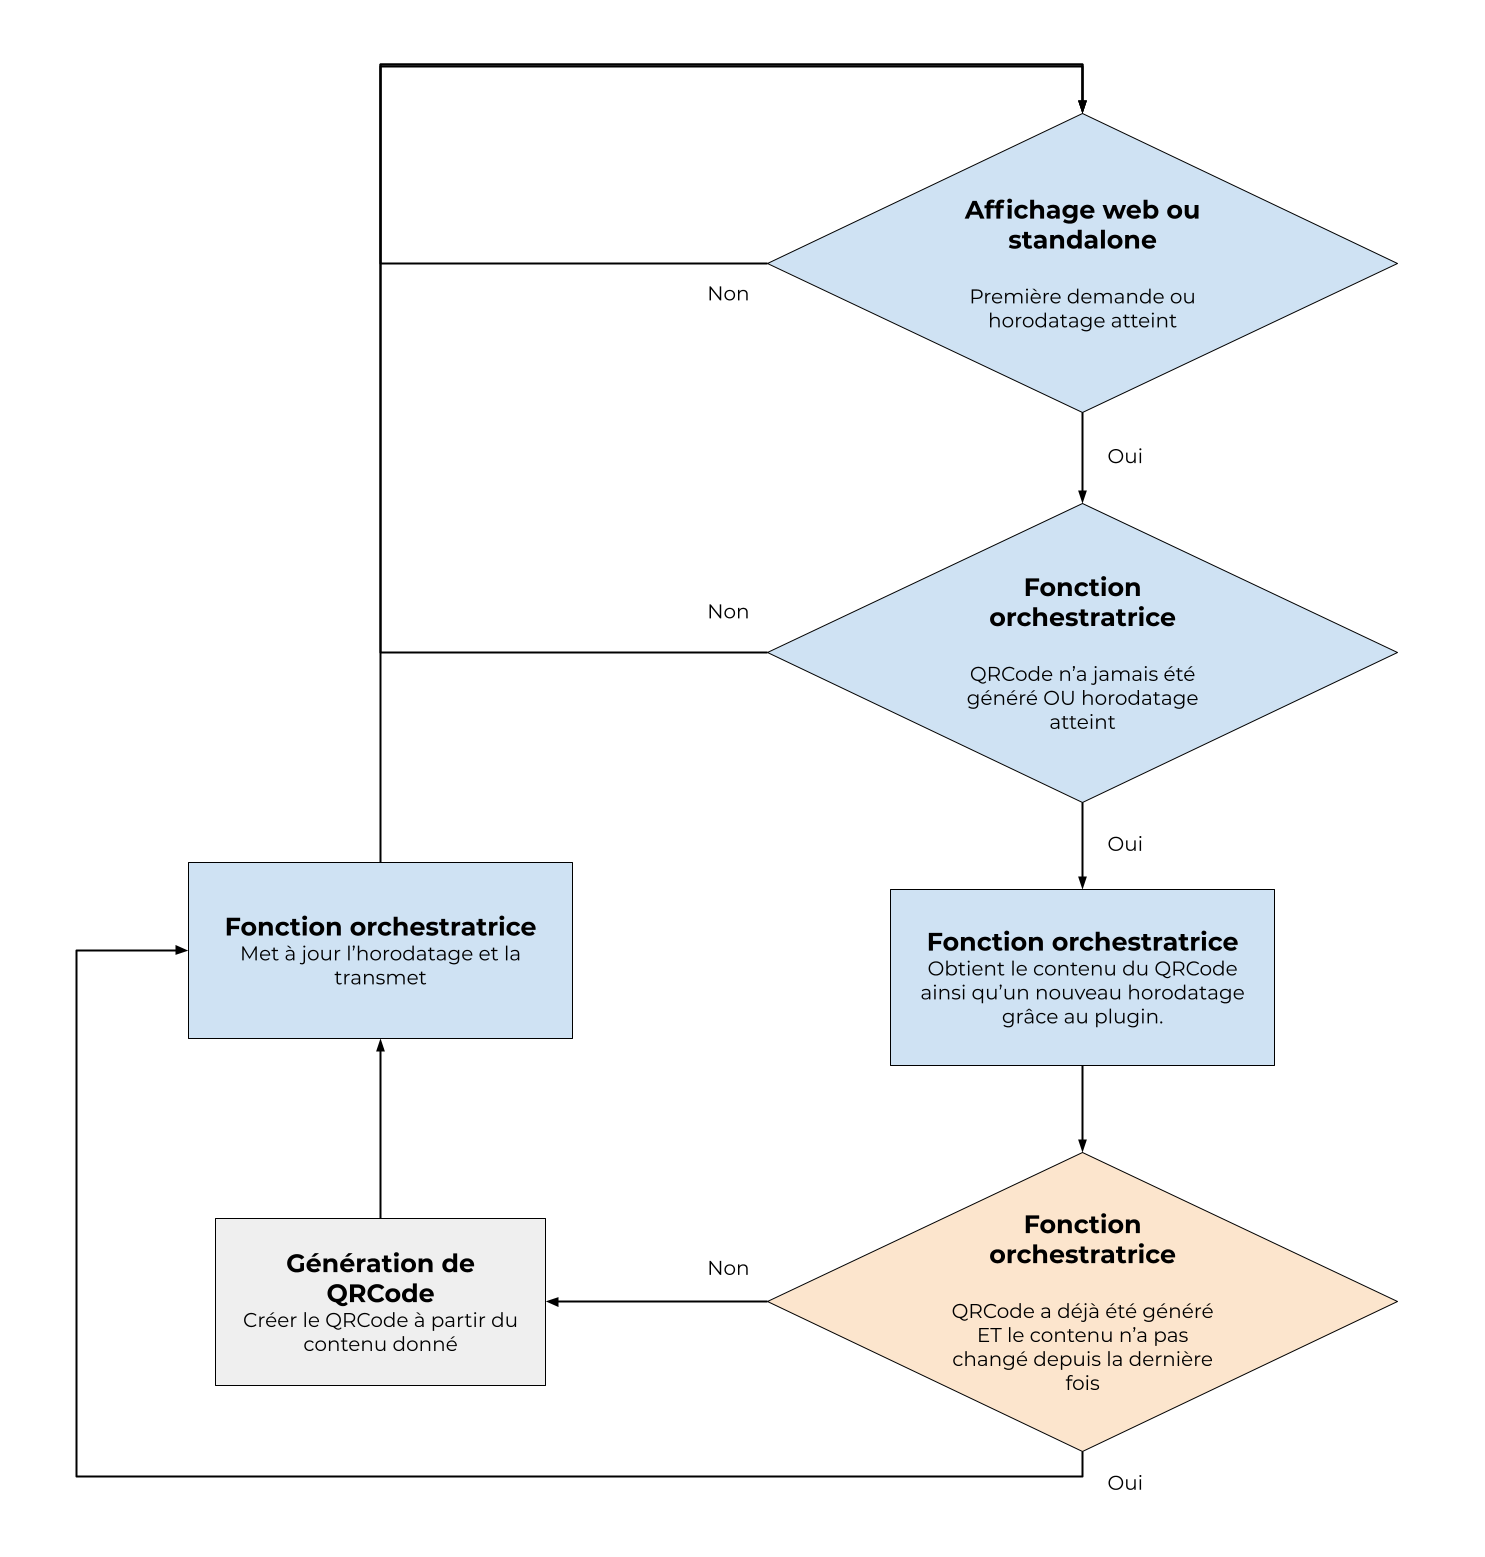
\includegraphics[width=.8\textwidth]{Logique_cache_2.png}
    \caption{Diagramme logique présentant comment l'utilisation de systèmes de cache par horodatage et par hash réduisent le nombre d'appels vers les plugins et la partie \textbf{Génération de QR code}. Ces deux systèmes sont expliqués de manière plus détaillée ci-dessous.}
\end{figure}

Deux systèmes coexistent :\\

\begin{itemize}

  \item \textbf{Cache temporel (bleu)} : les plugins définissent un horodatage. C'est-à-dire qu'en plus de fournir le contenu à mettre dans le QR code, le plugin doit indiquer un intervalle de rafraîchissement désiré (ex : 20 secondes, 5 minutes, 1 heure...). Cette méthode n'est pas sans rappeler les entêtes "Expires" utilisés en HTTP\footnote{Les entêtes "Expires" sont utilisées pour indiquer au navigateur du client que la ressource envoyée restera valide jusqu'à une certaine date. Cela évite notamment de constamment demander le même fichier de police de caractère, le même logo en haut de la page, les même feuilles de style CSS; qui sont toutes des ressources extrêmement statiques. Plus d'info : \url{https://developer.mozilla.org/en-US/docs/Web/HTTP/Headers/Expires}}. Cet horodatage est utilisé par l'\textbf{intermédiaire web} et l'\textbf{Affichage client web} pour limiter les demandes de calcul et de génération des QR codes, qui sont deux opérations lourdes de ce système.\\
  \newpage
  \item \textbf{Cache du contenu (orange)} : il est également possible de réduire d'avantage le nombre d'appels vers la fonction de \textbf{génération de QR code}. En effet, la \textbf{fonction orchestratrice} conserve dans un fichier JSON les contenus fournis par les plugins. Si après l'appel d'un plugin le contenu généré est le même que le contenu précédent, il n'est pas nécessaire de re-générer l'image de QR code.\\
  
\end{itemize}
\subsection{Dynamisme par redirection}

\noindent L'architecture de la version par redirection est similaire au fonctionnement du BackEnd+FrontEnd web vu précédemment. Les modifications apportées sont les suivantes :\\ 
\begin{itemize}
    \item Fonction orchestratrice : il est possible de générer les images de QR code dynamisme par redirection dans le dossier src/backEnd/Redirection pour tous les plugins en faisant la commande 'python OrchestratorFunction.py'.
    \item Fonction orchestratrice : le JSON de retour dans la partie frontEnd inclut maintenant le contenu du QR code.
    \item Affichage web : qrCodeDyn est la classe d'élément qui était déjà en place, il affiche le QR code. On a maintenant aussi qrCodeDynRedirection qui affiche le contenu à la place.
    \item Redirection.php (https://dynqr.r-entries.com/redirection.php?plugin=[insérer nom de plugin]) : c'est une page web qui prend en paramètre le nom du plugin et qui va générer une balise div avec la classe qrCodeDynRedirection si un nom de plugin lui est fourni, sinon affiche "Ce lien est invalide".\\
\end{itemize}

\noindent Également pour l'utilisation par redirection, il est possible d'utiliser la commande 

\noindent \verb|python OrchestratorFunction.py| sans paramètre. Cela permet de générer les QR codes statiques contenant le lien web pour accéder à la page de redirection.
\\

\section{Analyse du fonctionnement \& Tests}

\subsection{Tests d'encodage et de caractères}

%look
\noindent En écrivant nos tests unitaires pour la génération de QR code, nous nous sommes rendu compte qu'il y avait un problème avec la bibliothèque de décodage pyzbar 0.1.8. Nous avons pu illustrer le problème avec un fichier de tests simpliste. Le code ainsi que l'analyse des résultats est disponible en annexe \ref{bug_unicode}. Nous avons ouvert un ticket sur le dépôt GitHub de pyzbar (\url{https://github.com/NaturalHistoryMuseum/pyzbar/issues/95} consulté le 07/04/2021); nous sommes actuellement en attente d'une réponse.\\

\noindent Nous avons essayer d'installer d'autres bibliothèques Python pour le décodage des QR codes tel que qrtools 0.0.2 ou zbar. Cependant dans les deux cas, il est nécessaire d'installer Microsoft Visual C++ 14.0 Build Tools ce qui rend l'installation lourde, complexe et différente entre les systèmes Windows et Linux.\\

\noindent Devant ces difficultés, nous avons décider de ne pas vérifier les contenus Unicode dans nos tests unitaires de génération de QR code. L'encodage des caractères Unicode étant une extension du projet inital, et notre temps étant limité, nous avons trouvé cette résolution acceptable. Nous vérifions quand même qu'il n'y a pas d'erreur lors de l'encodage et création de l'image.

\subsection{Tests de consommation mémoire}
% TODO! 

%look

\noindent Pour nos tests de mémoire, nous avons utilisé la bibliothèque memory-profiler (0.58.0), une bibliothèque maintenue et mise à jour régulièrement depuis 2011 par fpedregosa (\url{https://github.com/pythonprofilers/memory_profiler} (consulté le 07/04/2021)).

\noindent L'enregistrement des consommations mémoires est effectué avec la commande suivante : \verb|mprof run <commande à executé>| et il est possible d'obtenir un diagramme pré-formaté en tapant la commande : \verb|mprof plot|

\noindent Avant de poser une valeur de base pour la consommation des programmes sous Python, nous allons tester un programme minimal (un "hello world").

\begin{figure}[H]
\begin{center}
  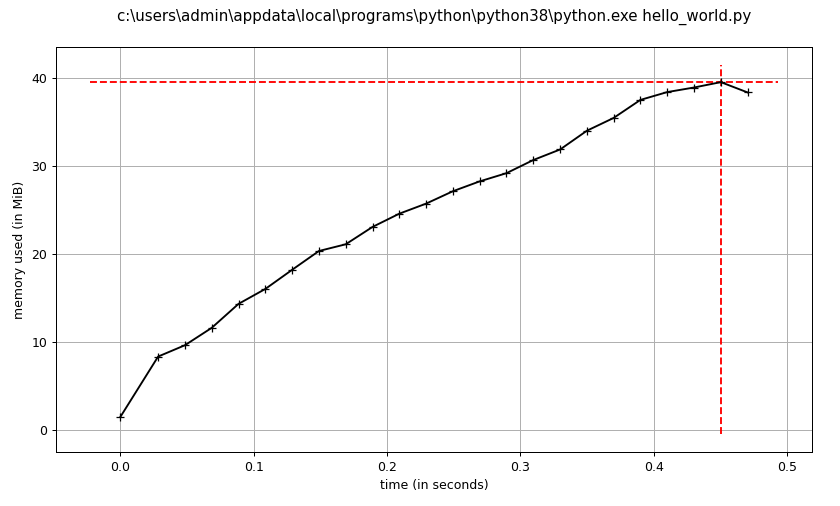
\includegraphics[width=.8\textwidth]{helloworld.png}
  \caption{On peut voir qu'un programme contenant uniquement print("hello world") consomme environ 39 Mo en mémoire.}
\end{center}
\end{figure}


\begin{figure}[H]
\begin{center}
  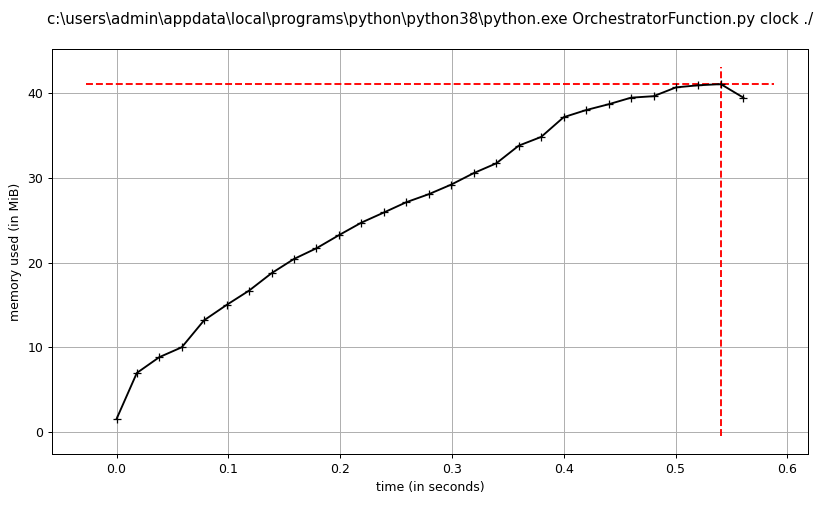
\includegraphics[width=.8\textwidth]{firstGeneration.png}
  \caption{Premier lancement de la fonction orchestratrice, première génération du plugin clock (voir \ref{clock} pour plus de détail sur ce plugin). On peut voir que l'exécution dure environ 0.55 secondes, la mémoire atteint un pic à 41 Mo.}
\end{center}
\end{figure}

\noindent Notre fonction orchestratrice est uniquement 1 à 2 Mo plus consommateur en mémoire qu'un hello world. Nous avons voulu calculer la taille en mémoire d'une image de QR code afin de confirmer que ces résultats sont cohérents : l'image produite pour le plugin clock mesure 435 par 435 pixels, la consommation est donc de 189 Ko (l'image est encodée sur 1 bit par pixel). Donc en prenant en compte les coûts d'instanciation de nos objets QRCode et PluginReturn ainsi que la consommation des bilibothèques que nous utilisons, ce résultat semble cohérent.\\

\noindent Intéressons nous maintenant au programme d'Affichage Standalone.
Encore une fois, nous allons tester une fenêtre graphique minimal en Tkinter afin de connaître la consommation minimale d'un programme utilisant cette biblothèque graphique.

\begin{figure}[H]
\begin{center}
  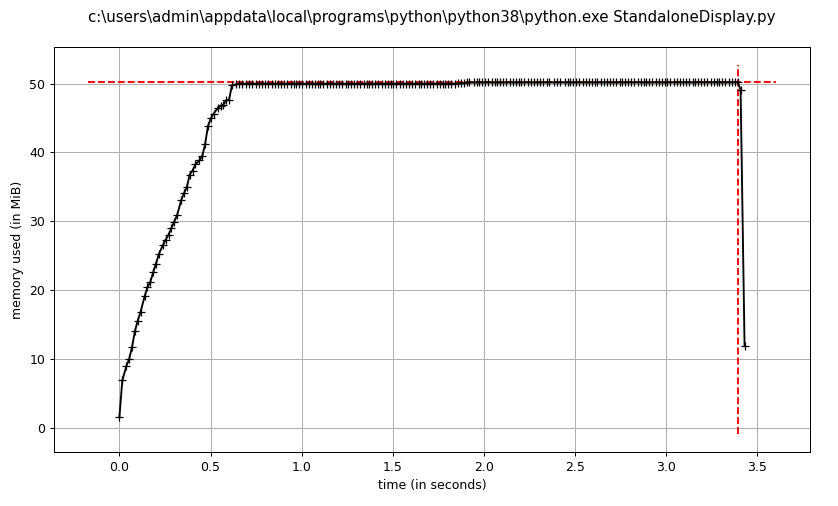
\includegraphics[width=.8\textwidth]{tkinter.png}
  \caption{On peut voir que ce programme affichant une fenêtre graphique Tkinter vide consomme environ 50 Mo.}
\end{center}
\end{figure}


\begin{figure}[H]
\begin{center}
  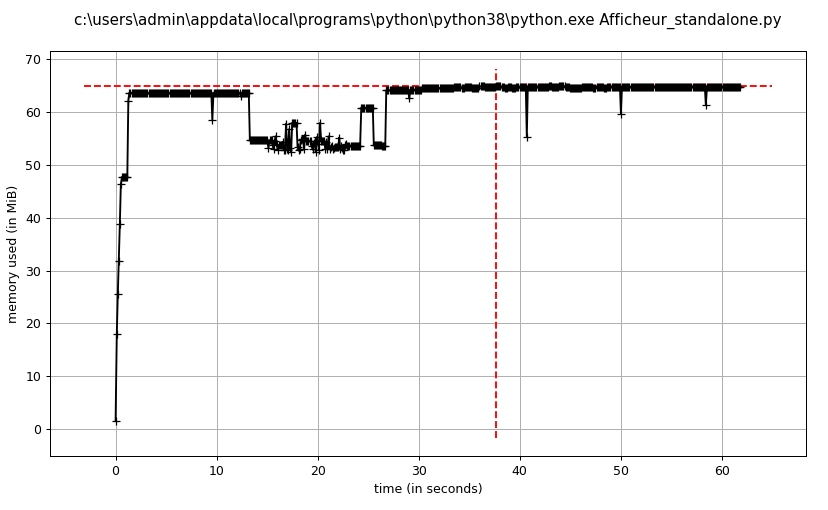
\includegraphics[width=.8\textwidth]{standalone.png}
  \caption{Premier lancement de l'affichage standalone. On peut voir une consommation qui plafonne à 65 Mo soit 15 Mo de plus qu'un programme Tkinter minimal.}
\end{center}
\end{figure}
\newpage
\noindent Il est important de noter que cette courbe de consommation de mémoire ne comprend pas la consommation de la fonction orchestratrice.
Il y a plusieurs phases : de 0 à 12, le programme se lance et affiche le plugin clock qui se rafraîchit toutes les secondes. De 12 à 27 secondes, l'utilisateur change frénétiquement la taille de fenêtre ce qui génère de nombreux redimensionnements de l'image. De 27 secondes jusqu'à la fin, l'utilisateur modifie aussi vite que possible le plugin sélectionné et active désactive le mode redirection.
On peut voir que la consommation est constante, fixée à 65 Mo. La seule période où la consommation varie est lorsque l'utilisateur redimensionne la fenêtre. 

\begin{figure}[H]
\begin{center}
  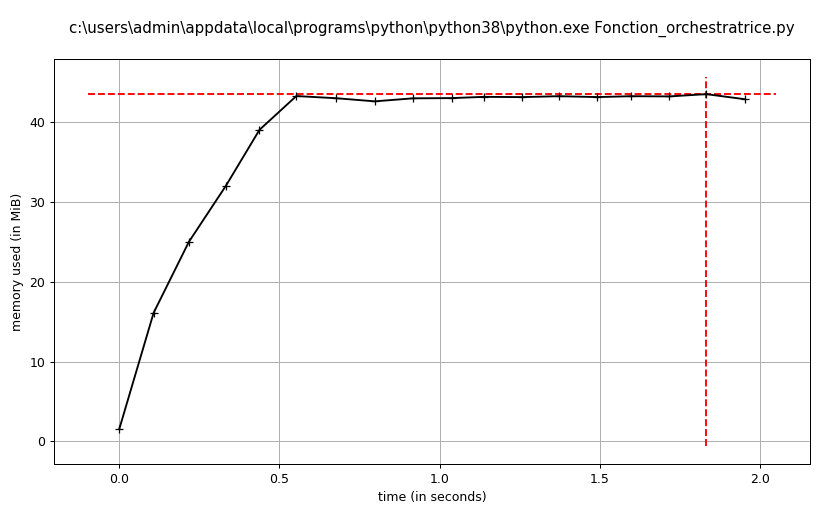
\includegraphics[width=.8\textwidth]{redirectionImageGeneration.png}
  \caption{Lancement du programme Fonction orchestratrice sans argument pour la génération des images de QR code à dynamisme par redirection. Pour ce test, 20 plugins ont été ajoutés dans le dossier Plugin. On peut voir que la consommation de mémoire reste constante à 42 Mo.}
\end{center}
\end{figure}

\subsection{Test de couverture des tests unitaires}

\noindent Pour nos tests de couverture, nous avons utilisé CoveragePy (\url{https://github.com/nedbat/coveragepy} consulté le 06/04/2021). Voici les résultats pour les tests unitaires sur la fonction de génération de QR code.

\noindent \begin{longtable}{ | m{.45\textwidth} | m{.15\textwidth} | m{.31\textwidth} | } 
\hline
\textbf{Name} & \textbf{Cover} & \textbf{Missing} 
\hline
backEnd/QrCode\_Generation.py & 95\% & 70-71
\hline
backEnd/OrchestratorFunction.py & 89\% & 73-75, 148-157
\hline
\end{longtable}

\noindent Nous pouvons constater que nos tests de la fonction Génération QR code couvre quasiment l'intégralité du code. De plus, les lignes 70 et 71 correspondent à la gestion d'une exception inconnue lors de la génération du QR code. 
Pour les tests de la fonction orchestratrice, les lignes 61-63 correspondent un try catch qui effectue de nouveau une sauvegarde du fichier cache.json dans le cas où le chargement de l'ancien fichier de cache aurait échoué .
Les lignes 131-140 correspondent à la section if \_\_name\_\_ == "\_\_main\_\_", une partie de code qui est exécuté uniquement si le fichier est lancé directement (ici le fichier est importé).

\subsection{Test de parallélisme web et performances}
\noindent Afin de tester les capacités de notre système à supporter plusieurs visiteurs sur une page possédant un QR code dynamique, nous avons ouvert 26 fenêtres du navigateur web Firefox\footnote{Au cas où la question ce pose, ouvrir 26 fenêtres crée bien 26 instances indépendante de l'application JavaScript exécuté. Nous en avons eu la confirmation lorsque nous avons commencé à modifier l'Afficheur client web, il était nécessaire de rafraîchir chaque fenêtre afin de rafraîchir le script utilisé.} sur une même machine avec pour URL notre site de test (\url{https://dynqr.r-entries.com/} consulté le 08/04/2021). Le QR code sélectionné était le plugin "clock" (voir \ref{clock} pour plus de détail sur ce plugin), avec un intervalle de rafraîchissement fixé à 3 secondes. Nous avons choisi cet intervalle car nous considérons cette valeur comme étant le minimum nécessaire pour scanner le QR code depuis un téléphone. Le serveur web tourne sur une machine virtuel avec 1 Go de mémoire vive et 1 vCPU. L'hyperviseur est un VMware ESXi 6.7.0 tournant sur un OptiPlex 7020. Le processeur étant un Intel(R) Core(TM) i5-4590 CPU cadencé à 3.30GHz (4 coeurs, 4 threads), 1vCPU serait l'équivalent d'un quart de la puissance de ce processeur. Cependant, comme notre programme Python n'est pas multi-threaded, la différence entre 1vCPU et le processeur entier reste limité.\\

\noindent Lorsque nous avons commencé ce test, nous avons ouvert seulement quelques navigateurs avant de voir un problème majeur : notre système n'ayant pas de système de protection contre la lecture ou écrite concurrence, si le fichier JSON ou l'image de QR code est modifiée pendant qu'un autre processus est en train d'essayer de le lire, cela a pour effet que la lecture est impossible. Dans le cas où l'image ne pouvait pas être lue, l'utilisateur se retrouvait avec une erreur à l'affichage jusqu'au prochain rafraîchissement. Dans le cas où le JSON ne pouvait pas être lu, l'afficheur client web ne pouvait pas récupérer l'intervalle de rafraîchissement et donc la boucle d'exécution s'arrêtait.\\

\noindent Nous avons fixé le problème de lecture du l'image en exécutant une fonction lorsque l'image n'a pas pu être chargée. Celle-ci va à nouveau essayer de charger l'image. La latence entre les deux tentatives est généralement suffisamment faible pour ne pas être visible par l'utilisateur.\\

\noindent Pour le problème de lecture du fichier JSON, nous avons fixé un intervalle de rafraîchissement par défaut à 10 secondes qui est utilisé en cas d'incapacité à lire l'intervalle fournis par le backEnd.

\noindent Un autre problème a été découvert, cette fois dans la partie backEnd. Encore une fois, il n'y a pas de système de gestion des lectures/écritures concurrentes. Ainsi, le fichier cache.json devenait parfois corrompu et illisible. Avant de détecter le problème, nous avons mis en place un test avec le plugin clock avec un rafraichissement à 3 secondes, 15 clients web en parallèle. Pendant les 25 minutes de ce tests, le fichier cache.json a été corrompu 49 fois (nous réinitialisions le fichier à chaque corruption afin que le test puisse continuer). La solution pour résoudre ce problème de lectures/écritures concurrentes est d'utiliser une bibliothèque de verrouillage de fichier. Nous avons choisi filelock 3.0.12 (\url{https://pypi.org/project/filelock} consulté le 09/04/2021) pour sa simplicité d'installation et d'utilisation. De plus il est compatible multi-os. Après avoir mis en place ce système, le fichier cache.json n'a jamais été corrompu sous les mêmes conditions que le test antérieur.\\

\noindent L'utilisation des verrous de fichier apportent un autre comportement intéressant : si l'on imagine x visiteurs connectés à la page web comportant un QR code dynamique, à partir de l'instant où le QR code atteint son horodatage de rafraîchissement, les navigateurs des visiteurs vont plus ou moins en même temps faire une demande au backEnd.\\ Le premier arrivé va verrouiller le fichier de cache ce qui va mettre en attente les autres jusqu'à ce que le fichier cache soit enregistré. A cet instant, les autres threads vont lire le fichier de cache, voir que le QR code est encore valide et stopper l'exécution presque instantanément. Nous avons donc une garantie que seul le premier thread effectue le travail sur une période de rafraîchissement donnée.\\

\begin{figure}[H]
\begin{center}
  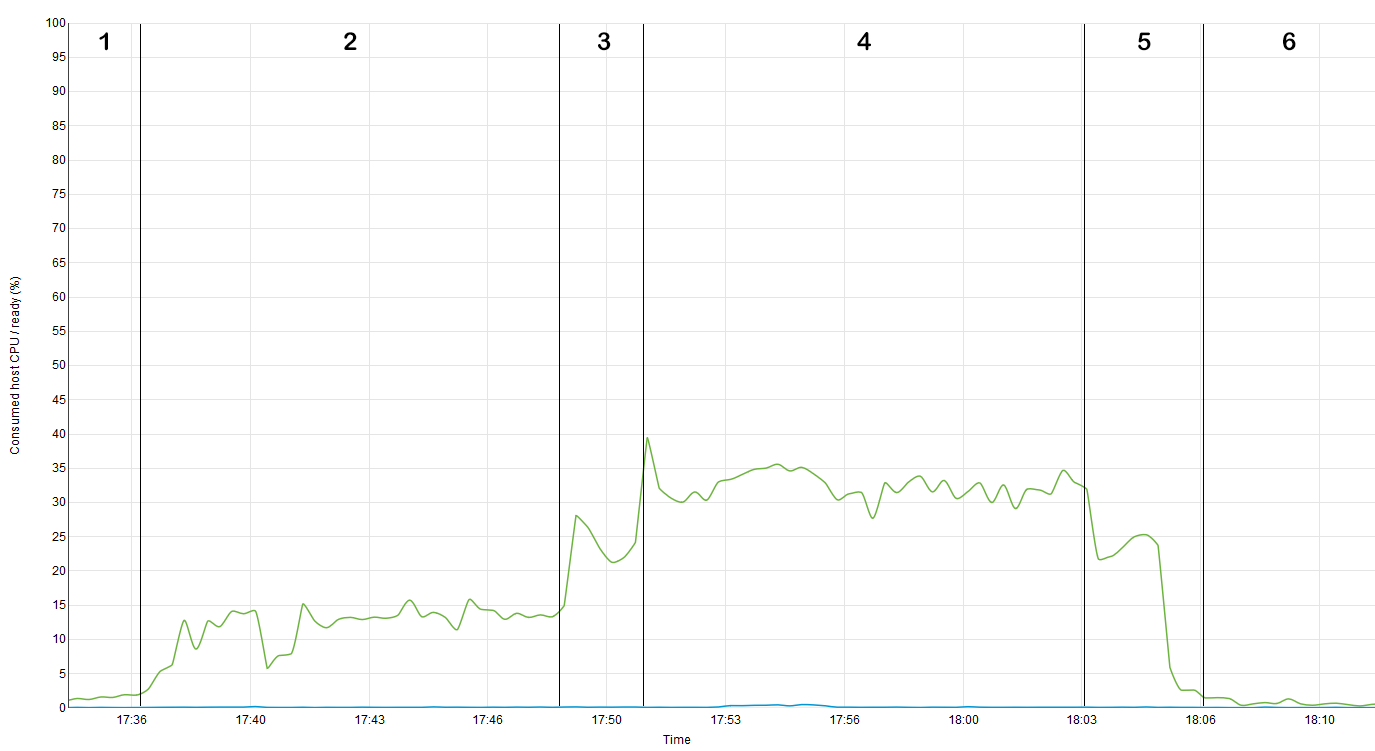
\includegraphics[width=.8\textwidth]{webparal.png}
  \caption{Le diagramme est fourni par l'interface web de VMware ESXi. L'axe horizontal est le temps. L'axe vertical est l'utilisation CPU de la machine virtuelle. Il y a 5 phases : (1) aucun visiteur, (2) 10 visiteurs pendant environ 10 minutes, (3) transition vers 26 visiteurs, (4) 26 visiteurs pendant environ 10 minutes, (5) transition de 26 visiteurs à 0 visiteurs, (6) aucun visiteur.}
\end{center}
\end{figure}

\noindent Les résultats montrent une utilisation processeur de 12\% pour 10 visiteurs (environ 1,2\% par visiteur) et 32\% pour 26 visiteurs (environ 1,23\% par visiteur). Avec seulement deux points de référence, cela reste approximatif que d'essayer de définir l'utilisation processeur suivant le nombre d'utilisateurs. En supposant que ce ratio est relativement linéaire, nous aurions un maximum théorique de 80 utilisateurs en parallèle sous ces conditions. Si l'exploitant souhaite diminuer l'utilisation processeur/augmenter le nombre de visiteurs maximal, il peut soit investir dans un système informatique plus performant, ou augmenter l'intervalle de temps entre deux rafraîchissement.



\section{Conclusion}

\noindent \`A l'origine de ce projet, nous devions réaliser un programme permettant l'affichage de QR codes dynamiques obtenus à partir de plugins utilisateurs modulables (possibilité d'en ajouter, d'en retirer, d'en modifier...). L'affichage devait se faire sur navigateur web (emploi d'un serveur php) ou sur un simple programme standalone exécutable sur machine (Windows ou Linux).\\

\noindent Au terme de ce projet, nous avons réussi à implémenter une version Standalone en python3 qui permet l'affichage de QR codes dynamiques portable sous Windows 10 et Debian.\\
Nous avons également réalisé un afficheur web comme demandé par notre client.\\
En plus de ces deux versions ainsi que de leurs extensions que nous avons détaillé plus haut dans la partie Architecture, nous avons développé une version alternative du projet basée sur des QR codes dynamiques par redirection.\\
De plus, ces trois versions utilisent la même interface Back-End pour fonctionner, elles ont été testées, mais ont tout de même certaines limitations.

\subsection{Limitations}

\subsubsection{Versions de Python prises en charge}
\noindent Nous avons testé notre projet sur Python 3.6, 3.7, 3.8, 3.9. 
Notre client n'avait pas de préférence particulière vis-à-vis de la version de Python à utiliser, nous avons donc choisi de supporter toutes les versions qui sont dans la liste des "releases actives" sur la page de téléchargement officielle (\url{https://www.python.org/downloads/}. Cela exclue donc Python 2.X (la dernière version 2.7 a atteint sa fin de vie le 01/01/2020). De même pour les version antérieur à la 3.6 comme Python 3.5 (fin de vie le 05/09/2020) et Python 3.4 (fin de vie le 18/03/2020).

\subsubsection{Nombre de visiteurs en parallèle}
\noindent Nos tests de performances ont montrés que notre système fonctionnait raisonnablement bien avec une trentaine de visiteurs connectés en parallèle sur la même page web. De plus, l'intervalle de rafraîchissement choisi était de 3 secondes, ce que l'on considère comme étant la durée minimale pour scanner un QR code sur un smartphone. Cependant, le plugin utilisé (clock) est extrêmement simple, légèrement plus complexe qu'un "Hello world". Si nous avions utilisé un plugin au fonctionnement plus complexe (peut-être même un plugin qui fasse des requêtes web), nous aurions certainement trouvé des résultats plus médiocre.

\noindent Nous ne nous sommes peu souciés de la possibilité d'avoir plusieurs demandes au backEnd en parallèle dans notre architecture, ce qui a des effets imprévisibles sur la validité des fichiers de caches.

\noindent Dans l'hypothèse où ce système devait être utilisé sur une plateforme avec beaucoup plus de visiteurs journaliers, nous avons imaginé une extension (voir \ref{daemon}) qui permettrait de résoudre ces deux problèmes.

\subsubsection{Approche par dynamisme intégré}
\noindent Concernant les limitations de l'approche par dynamisme intégré, on retrouve trois éléments principaux qui sont :\\
\begin{itemize}

  \item Vis-à-vis des QR codes limités dans le temps, l'implémentation proposée permet uniquement de retirer l'image de l'écran (utilisation standalone) ou de la téléverser au client (utilisation dans un site web). Dans l'éventualité ou un utilisateur télécharge l'image, la prend en photo ou potentiellement la publie, il n'est pas possible d'empêcher quiconque de scanner et de visionner le contenu du QR code. Cette limitation n'est pas dûe à notre implémentation mais est intrinsèque au fonctionnement des QR codes par dynamisme intégré. Seul la version par redirection permet de contourner cette limitation.\\
  
  \item Pour une utilisation web, il est nécessaire de déposer du code PHP et JS pour gérer le dynamisme des QR codes. Cela restreint leurs utilisations aux sites web dont on est administrateur : il n'est pas possible de les publier sur les réseaux sociaux et autres. Pour une utilisation standalone, il est bien sûr impossible de les imprimer, ou de les intégrer à un document PDF, PowerPoint, Word...\\

  \item Bien que PHP soit massivement utilisé sur les serveurs d'hébergement web, il existe d'autres frameworks tel que Asp .Net, Enyo, Ruby on Rails, NodeJs... Pour intégrer les QR codes sur un site utilisant une autre technologie que PHP, il serait nécessaire de réécrire une nouvelle version de l'\textbf{intermédiaire web}. Cela dit, son code est extrêmement simple, il ne fait que passer l'information entre le front-end et back-end.\\
  
\end{itemize}

\subsection{Extensions}
\label{ExtensionsProposées}
% BOF! Il manque peut-être d'autres extensions bonus qu'on a pas eu le temps de faire et que j'ai pas écrit ?
\noindent Il s'agit ici de lister un certain nombre de fonctionnalités supplémentaires réalisables qui dépassent le cadre du sujet donné par le client, et que nous n'avons pas eu le temps d'implémenter.\\

\subsubsection{Pouvoir personnaliser le style visuel du QR code}

    \begin{itemize}
        \item Changer la couleur de fond et couleur du QR code :\\
        Pour cette extension, il faut se pencher du côté du PluginReturn et du QrCode\_Generator. Lors de la génération d'un QR code il est possible de définir les couleurs via les arguments module\_color et background (voir fonction toPNG).\\ On peut imaginer un PluginReturn qui contiendrait en plus ces deux arguments, permettant de les transmettre au générateur.\\
        \item Ajouter un texte quelconque en dessous du QR code.\\
        \item Ajouter une icône au centre du QR code.\\
        Il est possible d'ajouter une image en petite dimension au centre ou même à un autre endroit du QR code à l'aide de PIL. Cependant cette méthode cache une partie du QR code, ce qui veut dire qu'il vaut mieux générer un QR code avec niveau de correction d'erreur H. Cela permet d'avoir une image qui couvre jusqu'à 30\% du QR code sans en endommager le contenu\footnote{Plus d'infos ici :\\ \url{https://stackoverflow.com/questions/45481990/how-to-insert-logo-in-the-center-of-qrcode-in-python} (consulté le 07-04-2021)}.\\ 
    \end{itemize}
\subsubsection{Interface web pour la gestion des QR codes}
    
\noindent Remplacer le système de plugins par une interface graphique permettant de paramétrer le dynamisme d'un QR code. Cela permettrait notamment de sécuriser le système : l'exécution de code arbitraire\footnote{Code arbitraire est employé pour nommer une action à faire faire à une machine sans que le propriétaire soit d'accord. Plus d'info : \url{https://en.wikipedia.org/wiki/Arbitrary\_code\_execution} (consulté le 12/02/2021)} est une faille importante dans l'éventualité où les plugins sont fournis par une personne tierce.\\

\newpage

\noindent En couplant l'implémentation du dynamisme par redirection avec une interface de paramétrage web, nous pourrions aborder l'idée de créer un service web permettant à des utilisateurs de créer un compte, créer/modifier des QR codes dynamiques, et les exporter. Nous pourrions par la suite imaginer différentes fonctionnalités comme par exemple : comptabiliser le nombre de fois où le QR code a été scanné (log des adresses IP se connectant à la page web, ou des systèmes plus avancés, basés sur "la capture d'empreinte digitale de navigateur" (voir la légalité et la demande potentielle de consentement)).

\subsubsection{Utilisation d'un daemon}
\label{daemon}

\noindent Lors de nos tests de parallélisme web, nous nous sommes rendus compte que la consommation CPU était plus ou moins proportionnelle à la quantité de visiteurs en parallèle.

\noindent Une méthode pour permettre un plus grand nombre de visiteurs serait d'utiliser un daemon (un service tournant en arrière plan) qui s'occuperait de toujours maintenir les images et fichier JSON de QR code à jour. Ainsi, le client web n'aura plus qu'à charger l'image actuellement disponible, de même pour le fichiers JSON. Plus besoin d'un intermédiaire web. L'avantage majeur est qu'il n'y a plus qu'un "utilisateur" du point de vue du backEnd. L'utilisation processeur de notre système serait également la même quelque soit le nombre de visiteurs web. L'inconvénient majeur est que le système va continuellement tourner en tâche de fond, même si aucun visiteur n'est présent.

\noindent En conclusion, le système actuellement en place est préférable pour un nombre faible et inconsistant de visiteurs, et ce nouveau système serait beaucoup plus efficace pour des sites avec de nombreux visiteurs.

\newpage

\section{Bibliographie}

\begin{itemize}

\item International Standard ISO/IEC 18004
Information technology — Automatic identification and data capture techniques — Bar code symbology — QR code\\
Disponible ici : \url{https://swisseduc.ch/informatik/theoretische\_informatik/qr\_codes/docs/qr\_standard.pdf} (consulté le 12/02/2021) \\

\item GitHub. 2021. bn4t/dynamic-qr. Disponible à : \url{https://github.com/bn4t/dynamic-qr} (consulté le 12/02/2021).\\
\item Burcea, C., 2021. Generating Barcodes and QR Codes in Java | Baeldung. Baeldung. Disponible à : \url{https://www.baeldung.com/java-generating-barcodes-qr-codes} (consulté le 12/02/2021).\\
\item Uqr.me. 2021. Dynamic QR Code Generator - Free, custom, tracking, with logo. Disponible à : \url{https://uqr.me/qr-code-generator} (consulté le 12/02/2021).\\
\item GitHub. 2021. giandonatoinverso/PHP-Dynamic-Qr-code. Disponible à : \url{https://github.com/giandonatoinverso/PHP-Dynamic-Qr-code} (consulté le 12/02/2021).\\
\item GitHub. 2021. hardeepnarang10/attendance-automation. Disponible à : \url{https://github.com/hardeepnarang10/attendance-automation} (consulté le 12/02/2021).\\
\item PyPI. 2021. PyQRCode. Disponible à : \url{https://pypi.org/project/PyQRCode} (consulté le 12/02/2021).\\
\item Qrd.by. 2021. QR Code Generator - Create Free QR Codes. Disponible à : \url{https://qrd.by/#dynamic-qr-code} (consulté le 12/02/2021).\\
\item PyPI. 2021. qrcode. Disponible à : \url{https://pypi.org/project/qrcode} (consulté le 12/02/2021).\\
\item PyPI. 2021. zbar. Disponible à : \url{https://pypi.org/project/zbar} (consulté le 12/02/2021).\\
\item GitHub. 2021. zxing/zxing. Disponible à : \url{https://github.com/zxing/zxing} (consulté le 12/02/2021).\\
\item PyPI. 2021. filelock 3.0.12. Disponible à : \url{https://pypi.org/project/filelock} (consulté le 09/04/2021).\\
\item PyPI. 2021. pycodestyle. Disponible à : \url{https://pypi.org/project/pycodestyle/}, (consulté le 09/04/2021).\\
\item Python. 2021. PEP8. Disponible à : \url{https://www.python.org/dev/peps/pep-0008/}, (consulté le 09/04/2021).

\iffalse

\item \url{https://uqr.me/qr-code-generator}\\
\item \url{https://qrd.by/#dynamic-qr-code}\\
\item \url{https://github.com/bn4t/dynamic-qr}\\
\item \url{https://github.com/giandonatoinverso/PHP-Dynamic-Qr-code}\\
\item \url{https://github.com/hardeepnarang10/attendance-automation}\\
\item \url{https://www.baeldung.com/java-generating-barcodes-qr-codes}\\
\item \url{https://pypi.org/project/qrcode}\\
\item \url{https://pypi.org/project/PyQRCode}\\
\item \url{https://github.com/zxing/zxing}\\
\item \url{https://pypi.org/project/zbar}\\

\fi


\end{itemize}

\newpage
\section{Annexe}

\subsection{Code du test de performance sous Java}
\noindent Ci-dessous le code utilisé pour nos tests comparatifs entre les performances de Java et de Python pour la génération des QR codes.

\noindent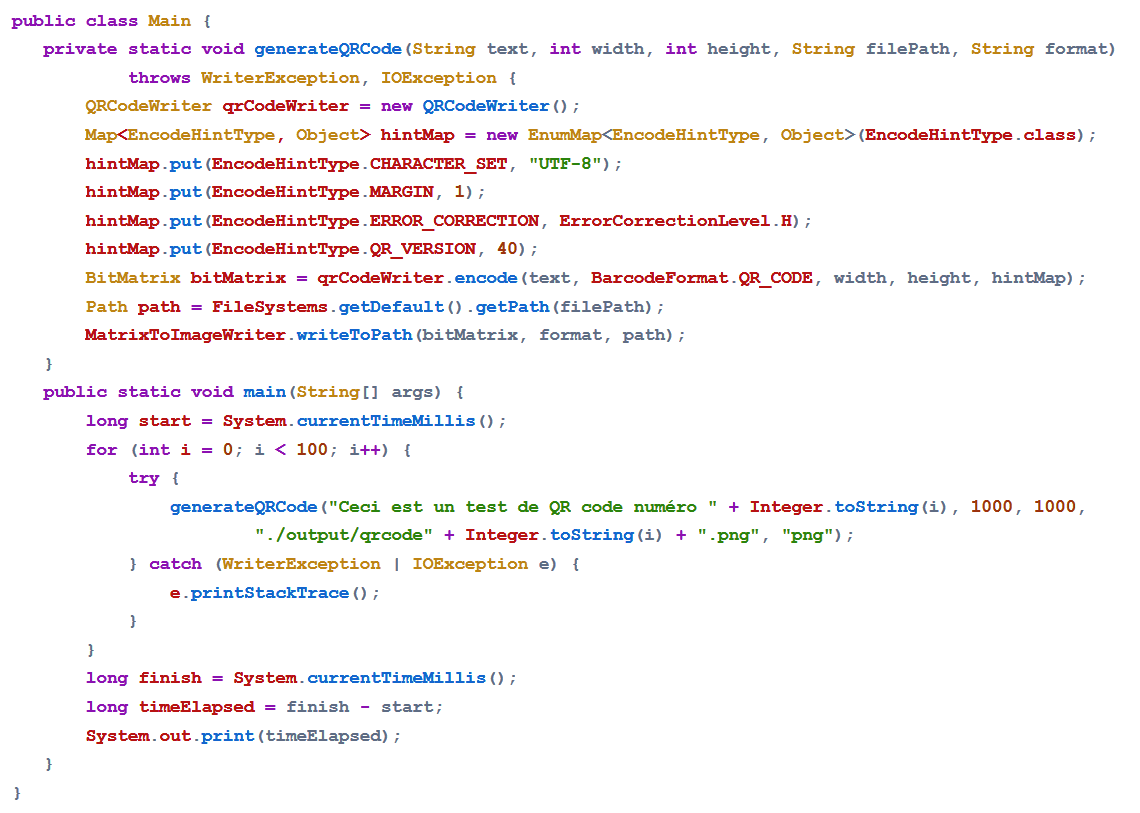
\includegraphics[width=\textwidth]{code-java.png}

\newpage
\subsection{Code du test de performance sous Python}
\noindent Un code beaucoup plus court pour le même algorithme. Veuillez ne pas prêter attention au nombre d'itérations qui est différente dans les deux programmes, nous les avons testés pour différents nombres d'itérations et il ne s'agit ici que de la dernière valeur entrée avant de faire une capture du code.
On peut également noter qu'il n'y a pas de méthode pour indiquer directement la taille de l'image finale. Nous pouvons la faire varier avec le paramètre "scale" qui définit la taille de chaque module.\\
La taille en pixels peut être calculée avec la formule suivante : ((version - 1) * 4 + 21) * scale.\\

\noindent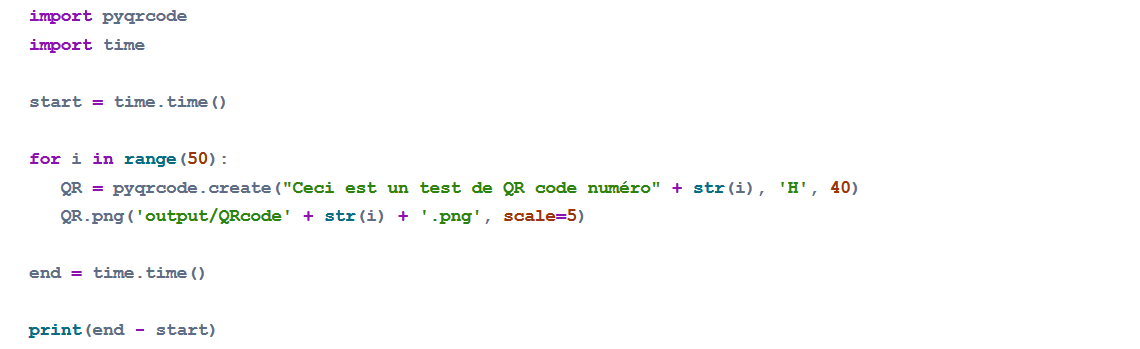
\includegraphics[width=\textwidth]{code-python.png}

\subsection{Exemple d'un plugin : clock.py }
\label{clock}
\begin{lstlisting}
from PluginReturn.PluginReturn import PluginReturn
import time

def getContent() -> PluginReturn:
    content = time.time()
    refreshTime = 5  # in s
    return PluginReturn(content, refreshTime)
\end{lstlisting}

\newpage

\subsection{Démonstration du bug Unicode avec pyzbar}
%look
\label{bug_unicode}
\begin{lstlisting}
import pyqrcode
import pyzbar.pyzbar
from PIL import Image

def encodeDecode(content):
    # Generate a QR code image from the content
    url = pyqrcode.create(content, encoding='utf-8')
    url.png('qrcode.png', scale=8)

    # Decode the QR code and retrieve the content
    decodedContent = pyzbar.pyzbar.decode(Image.open('qrcode.png'))[0].data

    # Compare with the original content
    if (decodedContent.decode('utf-8') == content):
        print("TEST OK with", content)
    else:
        print("TEST FAILED with", content)
    
encodeDecode('\u0100')
encodeDecode('\u0101')
encodeDecode('\u2133')
encodeDecode('\u0100\u2133')
encodeDecode('\u0101\u2133')
\end{lstlisting}

Caractères utilisés pour ce test :\\
\noindent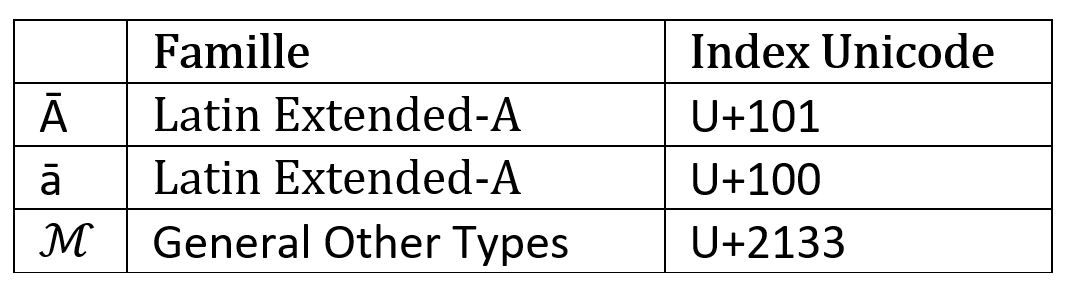
\includegraphics[width=.5\textwidth]{caractères.png}

\noindent Nous avons commencé par montrer qu'il n'avait pas de problème avec la bibliothèque de création de QR code (pyqrcode). Pour cela nous avons vérifié les images générées avec nos téléphones ainsi que la bibliothèque ZXing en Java. Les contenus des QR code correspondaient.

\noindent Voici maintenant le résultat de l'exécution du programme de test :\\
\noindent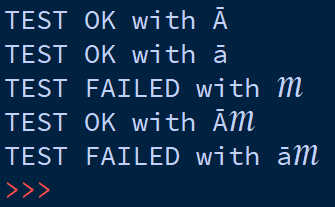
\includegraphics[width=.3\textwidth]{test_charactères.png}

\noindent Nous pouvons voir que les caractères 0100 et 0101 peuvent être décodés, mais pas le caractère 2133. Plus étonnant encore, la concaténation de 0100 et 2133 peut être décodée correctement mais pas 0101 et 2133.

\newpage

\subsection{Diagramme de Gantt}
% BOF! pas sûr du texte
\noindent Tout au long de la réalisation de ce projet, vous avons suivi ce diagramme de Gantt. On peut y voir que nous avons décidé de commencer par développer les parties qui sont en commun entre les deux approches. Après un retour auprès de notre client validant le suivi du projet, nous avons approfondi notre implémentation en proposant des tests et des extensions.\\ 
Il y a cependant eu des modifications par rapport à l'origine sur des choix d'extensions apportées, ainsi que sur les groupes chargés de réaliser telle ou telle tâche du diagramme.\\ 

\noindent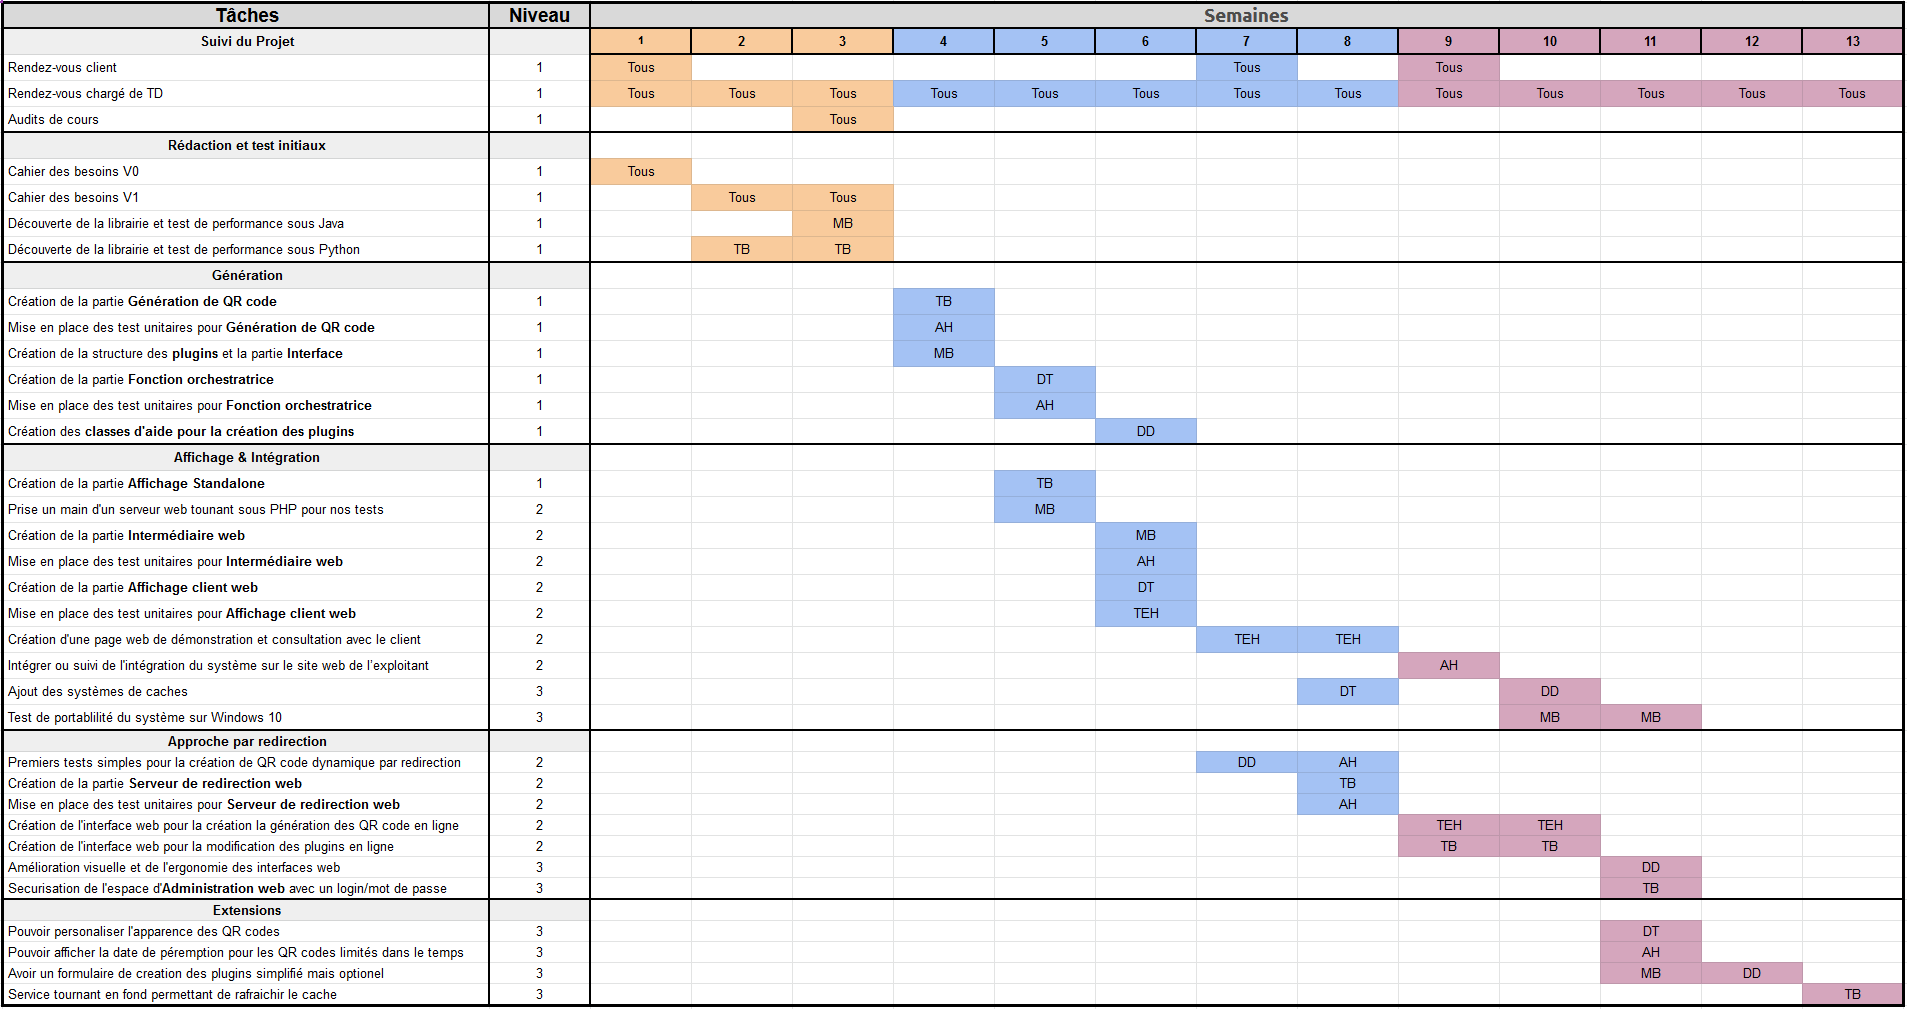
\includegraphics[width=\textwidth]{gantt.png}

\newpage

\subsection{Documentation utilisateur}
\begin{flushleft}

\textbf{Le dépôt git du projet est le suivant :}\\
\url{https://services.emi.u-bordeaux.fr/projet/git/qr-pdp-2021}\\
git clone https://services.emi.u-bordeaux.fr/projet/git/qr-pdp-2021\\
\end{flushleft}
\begin{flushleft}
\textbf{Installation nécessaire pour la version Standalone :}\\

\begin{enumerate}
    \item Python3.6 au minimum.
    \item Certaines librairies pip3 sont à installer :\\
    pip3 install pyqrcode;\\
    pip3 install pyzbar;\\
    sudo apt-get install zbar-tools (si problème avec linux)\\
    pip3 install pypng;\\
    pip3 install Pillow;\\
    pip3 install Tkinter\\
    sudo apt-get install python-tk (Si pip3 détecte pas Tkinter)\\
    pip3 install jsonschema\\
    pip3 install filelock\\
    
    Sur Windows, il faut utiliser python -m pip install <nom du module>
    \item Il ne reste plus qu'à aller dans qr-pdp-2021/src/frontEnd/standalone/ et taper cette commande :\\
    python3 StandaloneDisplay.py\\
    \item S'affiche alors à l'écran l'interface standalone.\\
    Pour quitter : echap ou fermer manuellement la fenêtre avec la croix.\\
    Pour changer le plugin affiché : cliquer sur le menu déroulant et choisir en cliquant sur le plugin voulu (au démarrage il est sur secret).\\
    Pour activer/désactiver le mode redirection : cocher/décocher la boite à cocher.\\
    \item Informations supplémentaires :\\
    Pour ajouter un <nom-plugin.py>, il faut avant de lancer le programme le mettre dans qr-pdp-2021/src/backEnd/Plugins/
    puis lancer l'afficheur standalone.\\
    L'ajout / retrait d'un plugin en cours d'exécution ne sera pas visible dans le menu déroulant (pas d'actualisation automatique).\\

    Il est possible de redimensionner la taille de la fenêtre qui au départ est à ScreenWidth/2 x ScreenHeight/2.\\
    La redimension est bloquée en dessous de la taille limite minimale (sinon ce serait illisible).\\

    La date et heure du prochain refresh de QR code ne s'affiche pas pour le mode redirection car l'image est statique.\\
\end{enumerate}
\end{flushleft}

\begin{flushleft}
\textbf{Installation nécessaire pour la version Web+Redirection :}\\
Il est nécessaire d'effectuer toutes les étapes de l'installation de la version Standalone pour cette version.\\
Il faudra installer en plus un serveur web. Pour ce tutoriel nous considérerons qu'il s'agit d'Apache2.\\
Il faut accorder les droits d'accès aux fichiers à www-data, le nom d'utilisateur qu'utilise Apache2 pour fonctionner : sudo chmod www-data:www-data -R à la racine du projet.\\

Par défaut, l'affichage des logs sont désactivés (question de sécurité), il est possible de les réactiver dans web\_intermediary.php pour du débogage.\\


Pour intégrer le système sur son site web, il faut placer le fichier src/frondEnd/web/web\_Intermediary.php sur une URL accessible depuis internet, de même pour  src/frontEnd/web/WebClientDisplay.js.

Dans le fichier WebClientDisplay.js, il faut changer la constante INTERMEDIAIRE\_URL en lui donnant comme valeur l'adresse de web\_Intermediary.php.


\end{flushleft}

\end{document}
